\documentclass{report}
\usepackage[a4paper,margin=3.5cm]{geometry}
\usepackage{cancel}
\usepackage{tikz}
\usepackage{amsmath,amsfonts,amssymb}
\usepackage{xcolor}
\usepackage{tcolorbox}
\usepackage{polynom}
\usepackage{wrapfig}
\usepackage{booktabs}
\usepackage{tabularx}
\usepackage{multicol}
\usepackage{hyperref}
\usepackage[ngerman]{babel}
\usepackage{tikz}
\usepackage{pgfplots}
\pgfplotsset{compat=1.18}
\usepackage{pstricks}
\usepackage{pst-plot}
\usepackage{textcomp}
\usepackage{import}
\usepackage{pdfpages}
%\usepackage{transparent}


\newcommand{\incfig}[2][1]{%
    \def\svgwidth{#1\columnwidth}
    \import{./figures/}{#2.pdf_tex}
}

\setlength{\parindent}{0pt}

\newcommand{\tbox}[2][0.8\linewidth]{
    \begin{center}
        \begin{tcolorbox}[colback=white, colframe=gray, width=#1]
                #2
        \end{tcolorbox}
    \end{center}}

\newcommand{\regel}[2][0.8\linewidth]{
    \begin{center}
        \begin{tcolorbox}[title=regel, colback=white, colframe=blue, width=#1]
                #2
        \end{tcolorbox}
    \end{center}}

\newcommand{\nt}[2][0.9\linewidth]{
    \begin{center}
        \begin{tcolorbox}[title=Notitz:, colback=white, colframe=gray, width=#1]
                #2
        \end{tcolorbox}
    \end{center}}


\newcommand{\ex}[2][\linewidth]{
    \begin{center}
        \begin{tcolorbox}[title=Beispiel:, colback=white, colframe=brown, width=#1]
                  #2
        \end{tcolorbox}
    \end{center}}


\newcommand{\q}[2][\linewidth]{
    \begin{center}
        \begin{tcolorbox}[title=Frage:, colback=white, colframe=purple, width=#1]
                  #2
        \end{tcolorbox}
    \end{center}}



\title{\Huge{Physik,}J1}
\author{\huge{Daniel Renschler}}
\date{Bis \today}


\begin{document}
\maketitle
\clearpage
\tableofcontents
\clearpage

% Spulen {{{
\section{P-lab, Spulen \date{17. Januar}}
\subsection{Unterricht}

Bei anderem Material in einer Spule ändert sich der Wiederstand (irgendwas mit
atomen in dem Material und Elektronen die in dem Material aneinander stoßen),
mit start genugem Netzteil kann man das aber umgehen udn die gleiche Leistung
durchbekommen. Eine andere größe die eine Rolle Spielt ist die Länge, und
Durchmesser der Spule.
Das Magnetfeld kann man messen mit einer… (satz geht gleich weiter, davor paar Formeln)
\[B=\frac{F}{I\cdot s} \text{Flussdichte B = Kraft=F, I=Stromstärke und s=Länge des Leiters}\]
Hall-Sonde macht Spannungsmessungen, diese kann man umrechnen in Flussdichte, angegeben in $T$.\\

%\begin{wrapfigure}{r}{5cm}
    %\centering
    %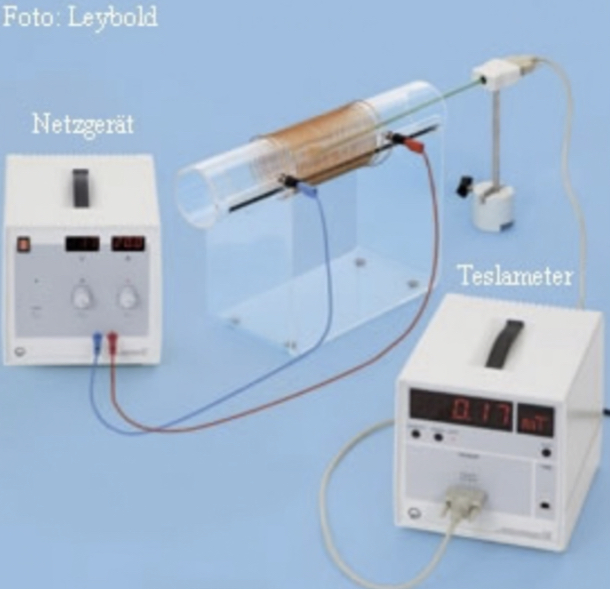
\includegraphics[width=0.25\textwidth]{physic-figures/Spule-Versuchsaufbau.jpg}
    %\caption{Versuchsaufbau}
    %\label{fig:physic-figures-spu-vers}
%\end{wrapfigure}


\noindent\textbf{Das Magnetfeld einer langen Spule}\\
Versuch: Magnetische Flussdichte einer langen Spule\\
Ziel des Veruchs: Wir möchten herausfinden wie die
magnetische Flussdichte $B$ einer langen Spule von der Windungszahl $n$ der
Spule, der lönge $l$ der Spule und der Stromstärke $I$ abhängt. (Hier abbildung
vom veruch) Mithilfe einer ``Hall-Sonde'' messen wir die magnetische
Flussidchte im Inneren einer mit Luft gefüllten langen Spule für verschiedene
Werte von $n, e$ und $I$. (nächste abbildung) Die Funktionsweise der Hall-Sonde
können wir erst später verstehen.\\

\noindent{\textbf{Messung A:} $n=30; l=0,35m$}
\begin{table}[htpb]
\begin{tabular}{|l|l|l|l}
\hline
I in A & B in mT & $\frac{B}{I}$ in $\frac{mT}{A}$ \\ \hline
3      & 0,30    & 0,100\\ \hline
6      & 0,61    & 0,102\\ \hline
9      & 0,88    & 0,988\\ \hline
\end{tabular}
\end{table}
$\implies \frac{B}{I}$= Konstant
= $B~I$ (B proportional)

\noindent{\textbf{Messung B:} $n=30; I=6A$}
\begin{table}[htpb]
\begin{tabular}{|l|l|l|l|l}
\hline
l in m &B in mT &In Feldstärke H    \\ \hline
0,1    &1,42    &1800\\ \hline
0,2    &0,90    &900\\ \hline
0,3    &0,67    &600\\ \hline
0,4    &0,46    &450\\ \hline
\end{tabular}
\end{table}

\noindent{Feldstärke $H = I \frac{n}{l}$}

\begin{table}[htpb]
\begin{tabular}{|l|l|l|l|l}
\hline
l in m &B in mT &Faktor zum nächsten \\ \hline
0,1    &1800  &$\frac{1}{2}$\\ \hline
0,2    &900   &$\frac{2}{3}$\\ \hline
0,3    &600   &$\frac{3}{4}$\\ \hline
0,4    &450   &$\frac{4}{5}$\\ \hline
0,5    &360   &$\frac{5}{6}$\\ \hline
0,6    &300   &$\frac{6}{7}$\\ \hline
0,7    &257,1 &...   \\ \hline
\end{tabular}
\end{table}
% }}}

% nochmal spulen{{{
\clearpage
\section{Weiter Spulen, von Konsti, \date{20. Januar}}
\subsection{Unterricht} Keine lange Spule $\to B=\frac{1}{l}$,$1=B\cdot l \to$
Antiproportional.\\ Aus  1. $B~I$ und aus\\ 2. $\frac{1}{l}$\\ wird
$B~l\cdot\frac{1}{l}$\\ $B~\frac{1}{l}$\\

$<=> \frac{B}{I\cdot\frac{1}{l}}$ = konstant = $M_0$ $\implies$ magnetische
Feldkonstante.
\[M_0=\frac{B}{I\cdot\frac{1}{l}}=\frac{0,3mT}{3\cdot\frac{1}{0,35m}}=0,00003s\] Bei
gleichzeitiger Verdopplung der Länge $l$ und der Windungszahl $n$ bleibt die
magnetische Flussdichte $B$ konstant.\\ $\implies B~l\cdot\frac{n}{l}$\\
$\implies B=M_0\cdot\frac{n}{l}\cdot l$


%\begin{minipage}{\textwidth}
%\centering
%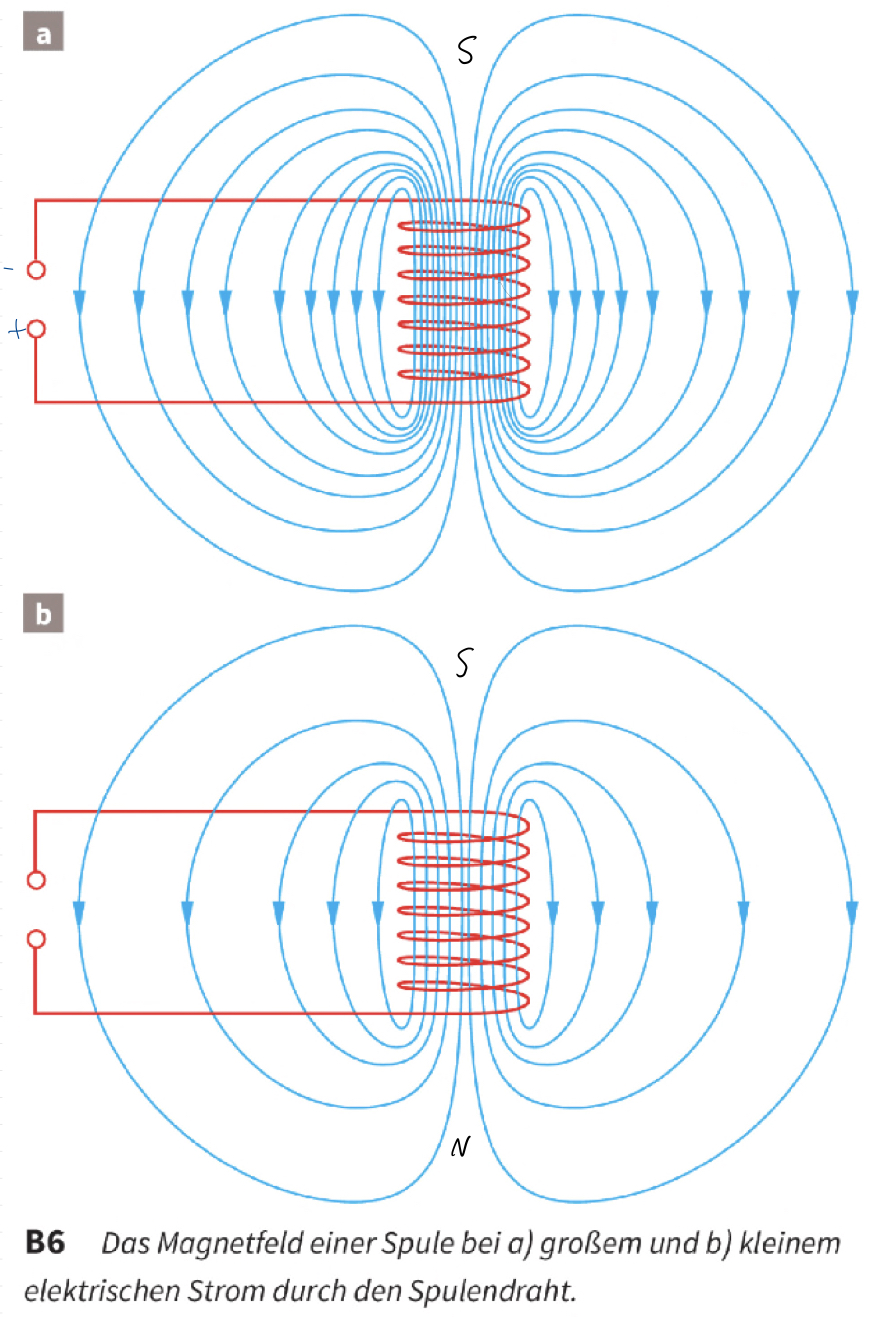
\includegraphics[width=0.2\textwidth]{/Users/daniel/docs/LaTeX/notes/physic-figures/Spule1.jpeg} 
%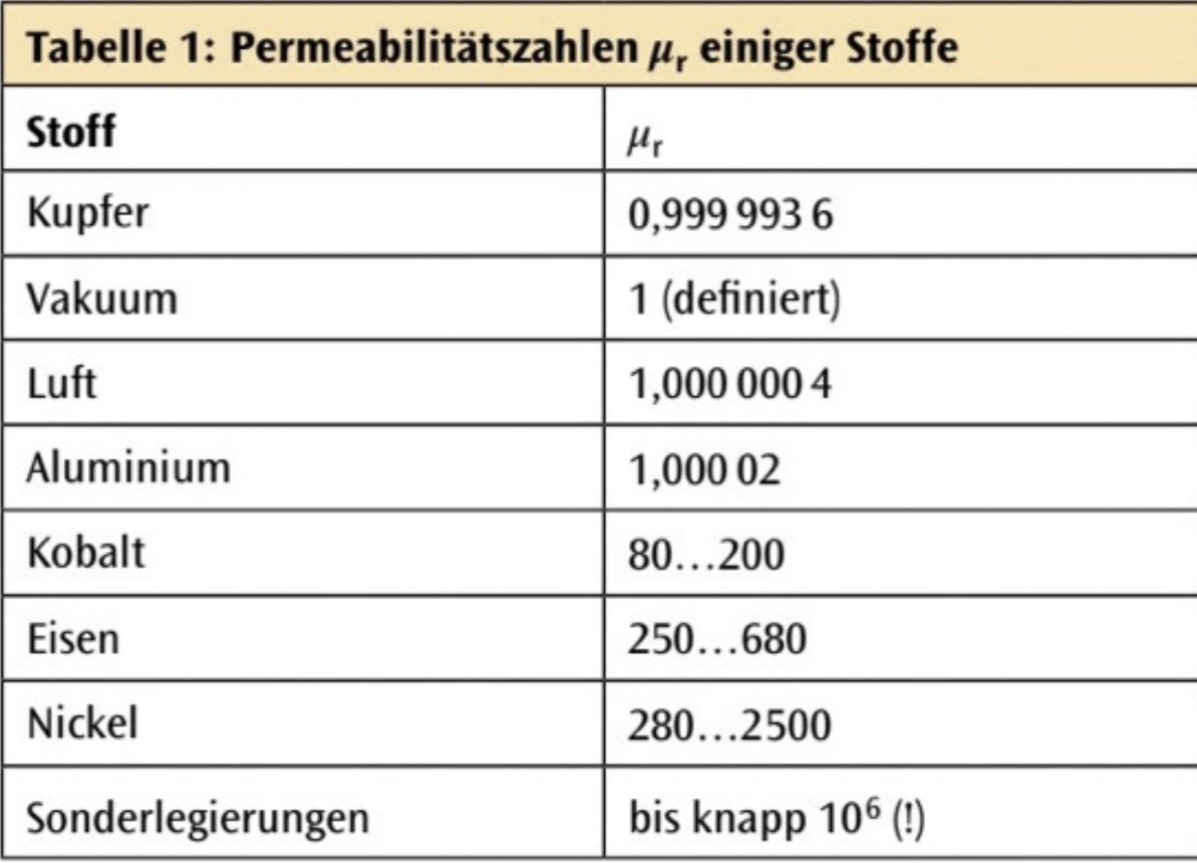
\includegraphics[width=0.4\textwidth]{/Users/daniel/docs/LaTeX/notes/physic-figures/Tabelle-Permeabilitatszahlen.jpg}
%\end{minipage}

Füllen wir die Spule mit einem Material (z.B. Eisen), so erhöht sich die
magnetische Flussdichte $B=\mu_0 \cdot Mr \cdot \frac{h}{l}\cdot I$ ($\mu$ ist die
Permeabilit\"atszahl)

%\begin{figure}[htpb] \centering
%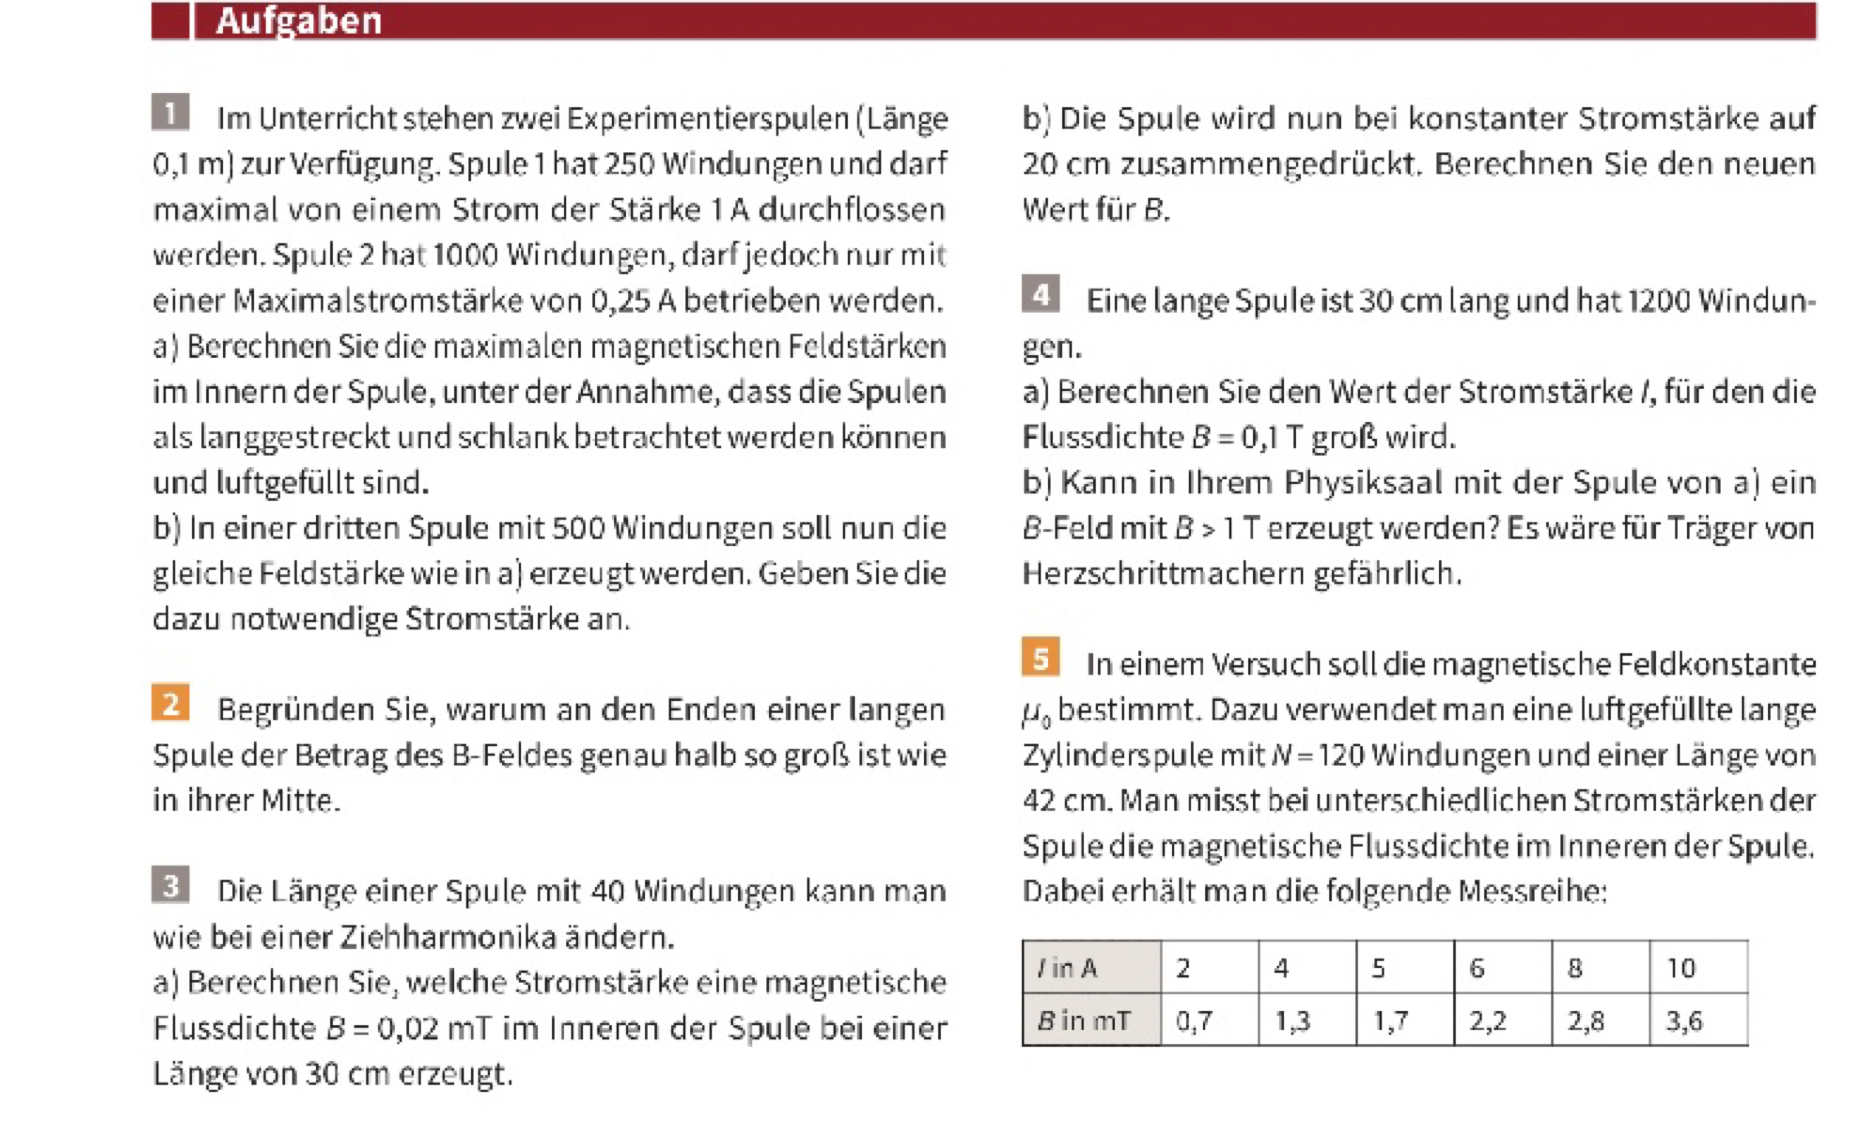
\includegraphics[width=0.8\textwidth]{/Users/daniel/docs/LaTeX/notes/physic-figures/Aufgaben1.jpeg}
%\caption{Aufgaben} \end{figure}

\[B=\mu_0\cdot\frac{n}{l}\cdot I\]
\textbf{1)}$B=1,2566\cdot 10^{-6}\cdot \frac{250}{0,1m}\cdot 1A=0,00314T=3,14mT$\\
\textbf{2)}$B=1,2566\cdot 10^{-6}\cdot \frac{1000}{0,1m}\cdot
0,25A=0,00314T=3,14mT$\\
$B=\mu_0 \cdot \frac{n}{l}\cdot l\implies \frac{B}{\mu_0\cdot \frac{n}{l}}=I\implies
I=\frac{0,00314T}{1,2566\cdot 10^{-6}\cdot \frac{500}{0,1m}}=0,4998A \thickapprox 0,5A$\\
\textbf{Nr.3}\\
\textbf{a)}$I=\frac{B}{\mu_0\cdot \frac{n}{l}}=\frac{0,02mT}{1,2566\cdot 10^{-6}\cdot \frac{40}{0,3m}}=119,37A$\\
\textbf{b)} $B=1,2566\cdot 10^{-6}\cdot \frac{40}{0,2m}\cdot 119,37A=0,03mT$\\ \textbf{Nr.
4}\\ \textbf{a)}
$I=\frac{B}{\mu_0\cdot \frac{n}{l}}=\frac{0,1T}{1,2566\cdot 10^{-6}\cdot \frac{1200}{0,3m}}=19,89A
\thickapprox 20A$\\ \textbf{Nr.5}\\
$\mu_0=\frac{B}{I\cdot \frac{n}{l}}=\frac{0,0007T}{2A\cdot \frac{120}{0,4m}=1,225\cdot 10^{-6}}$\\
% }}}

% Ka 2, Musterlosung {{{
\clearpage \section{Ka 2, Musterlösung, \date{23. Januar}}

%\textbf{Aufgabe 1a}\\ \begin{figure}[htpb] \centering
%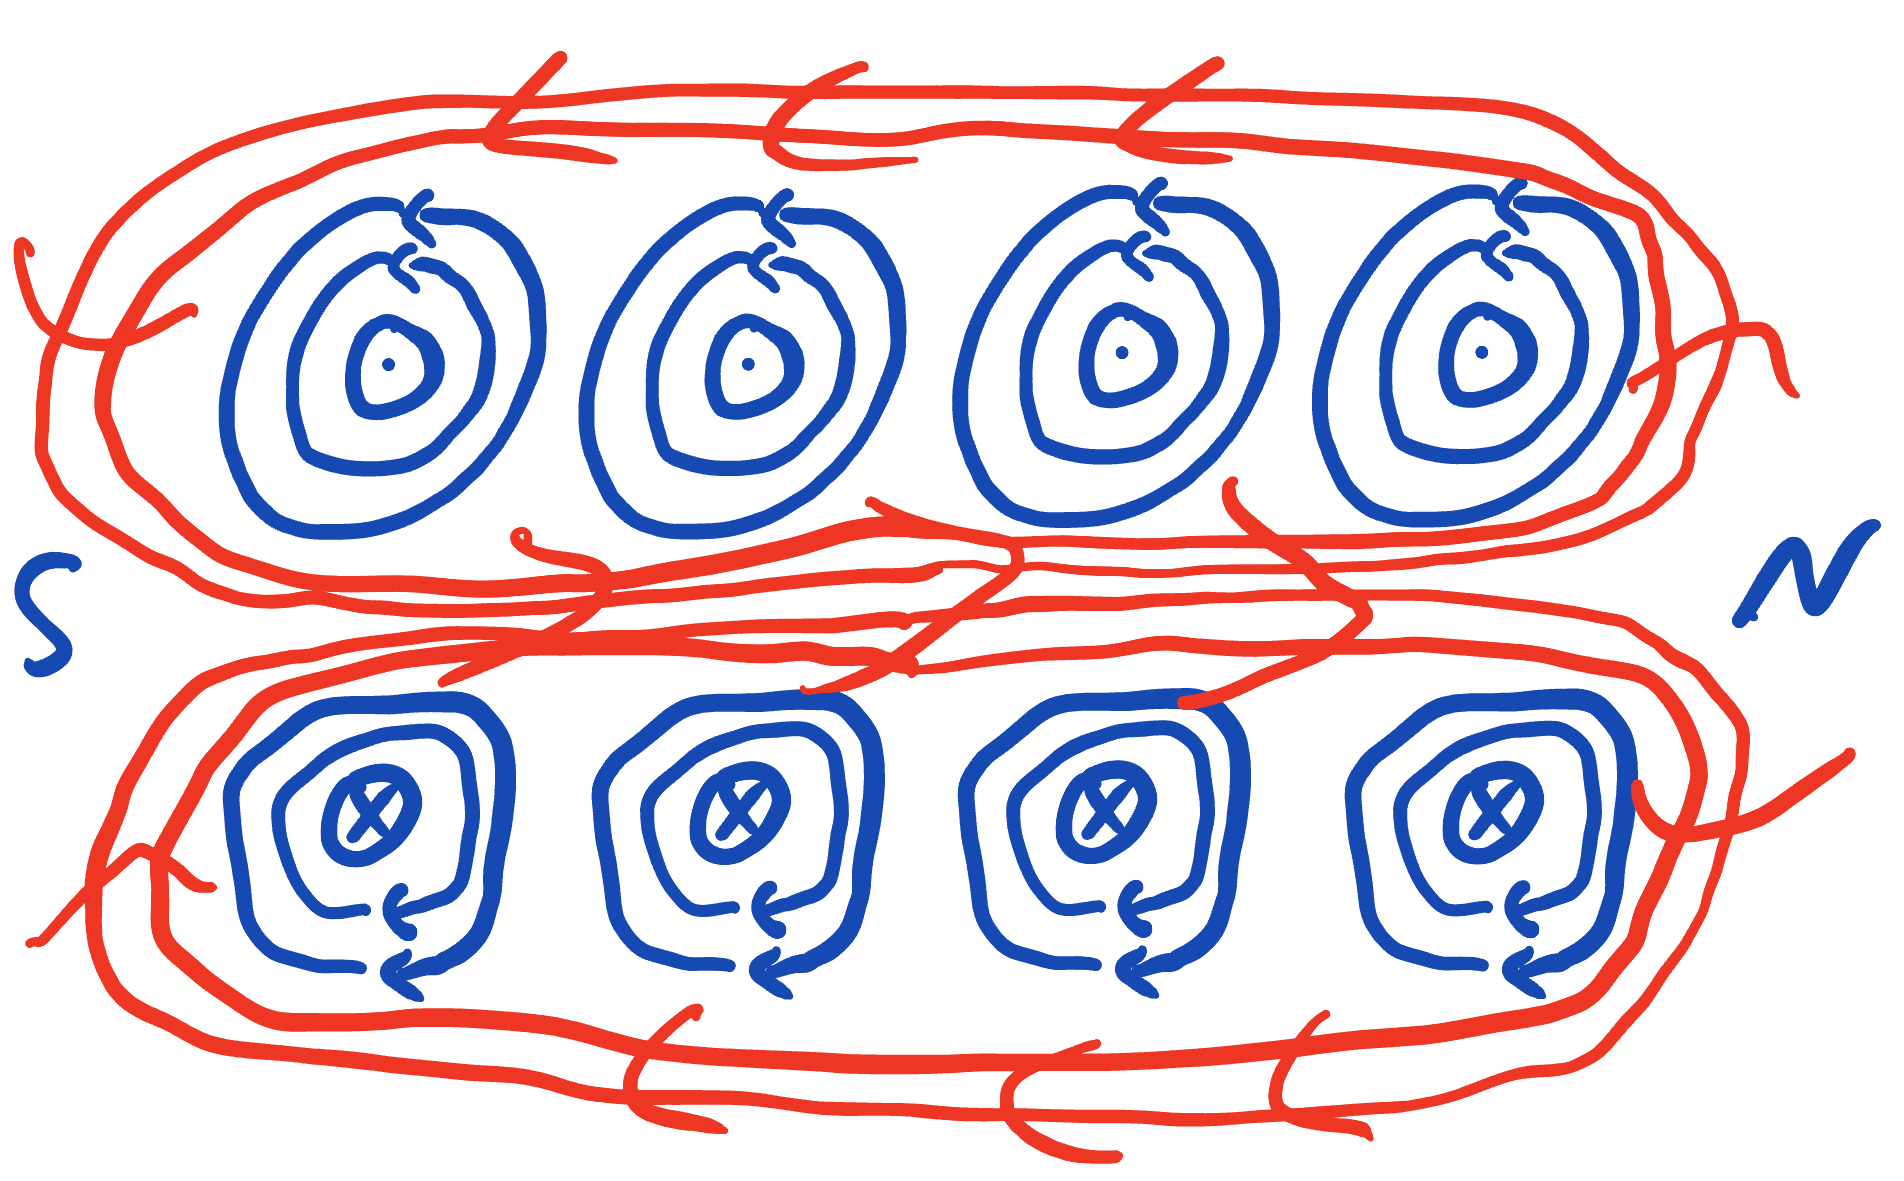
\includegraphics[width=0.35\textwidth]{physic-figures/ka-2-1a.jpeg}
%\caption{Magnetische Spule} \label{fig:physic-figures-ka-2-nr-1a}
%\end{figure}\\


\textbf{Aufgabe 2b} Nordpol ist rechts, Südpol ist links, weil bei einem
Magneten die äußeren Feldlinien von Nord nach Süd verlaufen. In der Spule
verbinden sie außen von rechts nach links, somit ist der Nordpol rechts und der
Südpol links.\\ \textbf{Aufgabe 1c} Abbildung 1b ist richtig. Wegen der rechten
Hand Regel muss der Daumen nach Süden zeigen. Die restlichen Finger zeigen die
Richtung des technischen Spulenstroms.


%\begin{figure}[htpb] \centering
%\includegraphics[width=0.35\textwidth]{physic-figures/ka-2-nr-2.png}
%\caption{Nr. 2 a} \label{fig:physic-figures-ka-2-nr-2} \end{figure}

\noindent \textbf{2 (b)} Der untere Körper ist der Eisenstab, da er direkt auf
die Indifferenzzone des oberen Magneten gerichtet ist und somit keine bzw. eine
sehr geringe Anzeihung erfährt, die je nach Masse des Stab nicht ausreichen
könnte um diesen anzuziehen. Somit fällt dieser runter.

\noindent\textbf{Aufgabe 3a} Anschluss $A_2$ = Pluspol, da Strom in technischer
Stromrichtung fließt, also von $A_2$ nach $A_1$. Laut der 3-Finger-Regel
verläuft die magnetische Wirkung ``in das Bild rein'' und somit wirkt die
Lorentzkraft nach unten auf den Leiter.\\ \textbf{Aufgabe 3b}\\ 1. Messreihe\\
$\frac{F}{I}\thickapprox 1,7 \longleftrightarrow$ konstant, proportional
$[F~I]$\\ 2. Messreihe\\ $\frac{F}{b}\approx 0,21 \longleftrightarrow$
konstant, proportional $[F~b]$\\ $\implies B=\frac{F}{I\cdot b}$, somit ist B der
Propitionalitätsfaktor\\
$B=\frac{F}{I\cdot b}=\frac{0,00034N}{2A\cdot 0,08m}=0,0021375T$\\ $\implies$ Der Wert
des Propitionalitätsfaktors ist 0,0021375T\\ \textbf{Aufgabe 3c} Er erhöht
sich.\\ \textbf{Aufgabe 4}\\ geg.: $V=\frac{2cm}{s}; e=1,6022\cdot 10^{19}C;
F_G=9,81\frac{N}{kg}; me=9,1093897\cdot 10^{-31}$\\ ges.: B\\ R:
\[B=\frac{F_G}{V_S\cdot e}=\frac{9,81\frac{N}{kg}\cdot 9,1093897\cdot 10^{-31}kg}{0,02\frac{m}{s}\cdot 1,6022\cdot 10^{-19}C}=3\cdot 10^{-9}T\]
$\implies$ Bei Bewegung in richtung Westen wirkt $F_G$ nach unten. Somit ist
die Richtung der Flussdichte laut 3-Finger-Regel nach Norden. \clearpage
% }}}

% Magnetfeld {{{
\section{Magnetfeld, \date{27.1.2023}}
\subsection{Unterricht} \textbf{a Zusammenfassung Buch Seiten 36-38:}\\ Der
magnetische Südpol liegt nicht am Nordpol, sondern in einer Inselgruppe im
Norden Kanadas und der magnetische Nordpol nicht am Südpol sondern südlich von
Australien auf Antarktika, die position ändert sich ständig. Magneticher Nord
und Südpol bilden auch die Drehachse, an der siche die Erde dreht. Die
Abweichung in genauigkeit von Kompassen nennt man Deklination. Die
rotationsachse ist mit dem Inklinationswinkel $\delta$ Sonnenwinde haben auch
Magnetfelder. Flussdichte des Erdmagnetfeldes: \[B=\frac{B_h}{\cos \delta}\]
$B_h$ ist die Ankatete zum Inklinationswinkel.

\noindent\textbf{b-Kontrollaufgabe}
%\begin{wrapfigure}{r}{5cm} \centering
%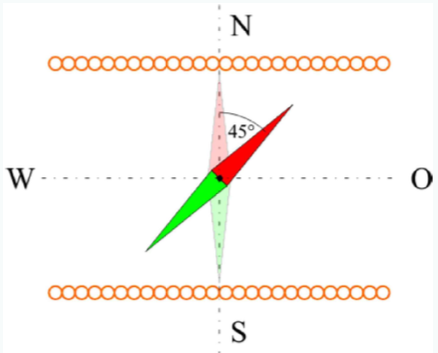
\includegraphics[width=0.4\textwidth]{physic-figures/magnetnadel.png}
%\caption{Magnetnadel} \label{fig:physic-figures-magnetnadel} \end{wrapfigure}

\textit{Eine lange Spule hat 3600 Windungen auf einer Länge von 60cm. Sie ist
so aufgestellt, dass ihre Achse in der magnetischen Ost-West-Richtung verläuft
(siehe Abbildung). In ihrer Mitte ist eine Magnetnadel in horizontaler Ebene
frei drehbar gelagert. Bei einem Spulenstrom von 24mA erfährt die Magnetnadel
eine Auslenkung von 45°.}\\

\noindent\textbf{a} Berechnen sie aus den Messwerten die horizontale Komponente
$B_h$ des Erdmagnetfeldes.\\ $\mu_0=1.2567\cdot 10^{-6}$ \[B_{sp}=B_h,
B_h=\mu_0\cdot \frac{n}{l}\cdot I \implies B_h=0,000190965T \implies 180,965\mu T\] Kann
nicht sein, da die maximale Stärke an den Polen nur ein drittel des Ergebnises
ist.

\noindent\textbf{b} Die Feldlinien des Erdmagnetfeldes treten am
Beobachtungsort unter einem Winkel von 67° (Inklinationswinkel) in den Erdboden
ein. Berechnen Sie aus diesen angaben den Betrag des Erdmagnetfeldes an diesem
Ort.\\ \[B=\frac{B_h}{\cos(67^\circ)}=463,149 \mu T\]

\subsection{Versuche} \subsection{Die elektrostatische Kraft E2-7}
%\begin{wrapfigure}{r}{3cm}
%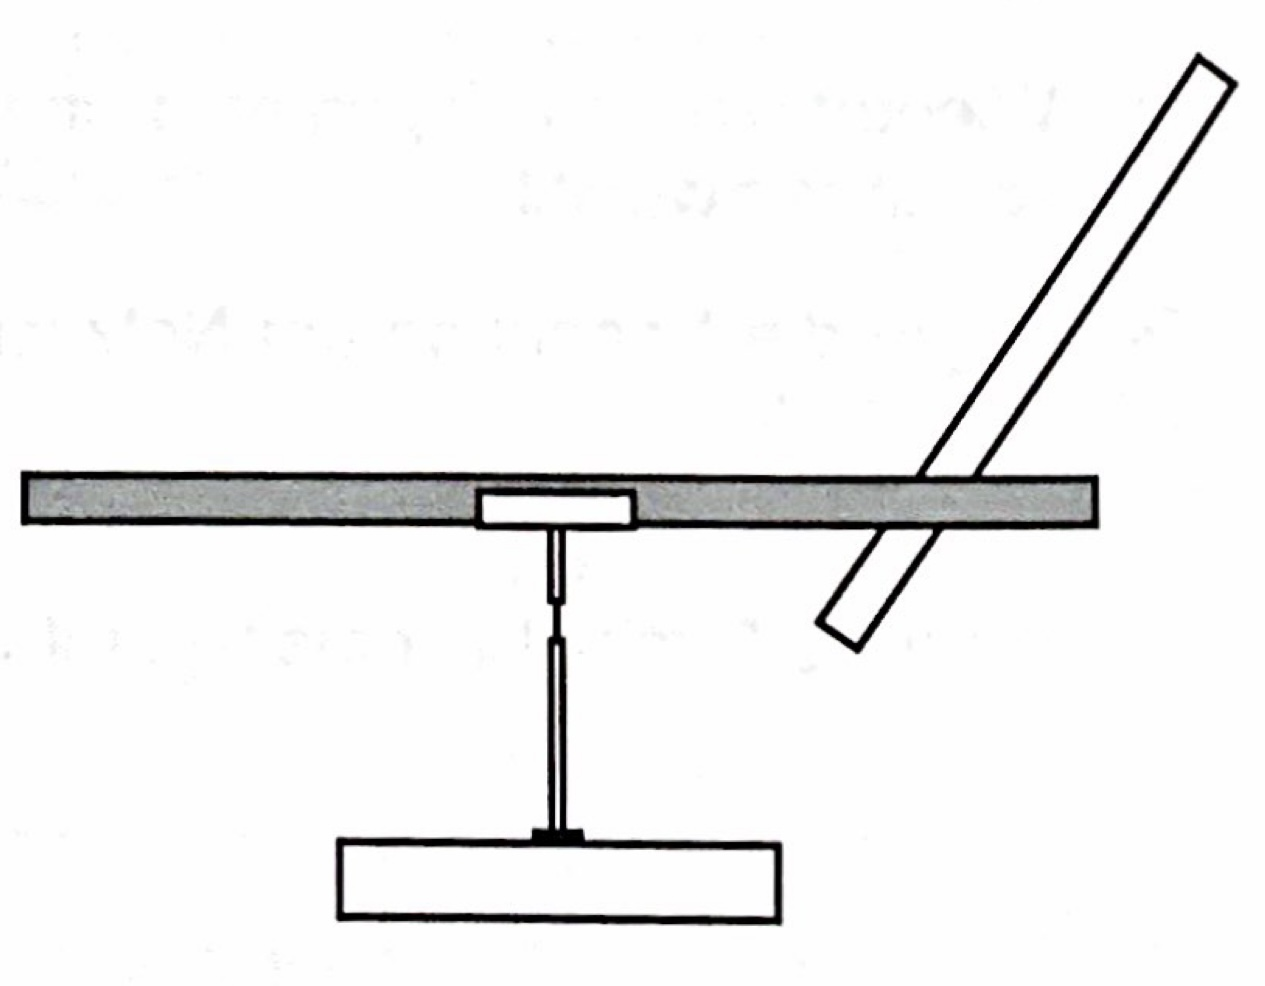
\includegraphics[width=0.2\textwidth]{physic-figures/elektrostatisch-1.jpeg}
%\caption{wie es halt heißt} \label{fig:physic-figures-elk-stat1}
%\end{wrapfigure}

\subsubsection{Einführung} Einige Erscheinungen der Elektrizität sind schon
seit dem Altertum bekannt. So berichtet beispielsweise THALES von Milet (um 600
v. Chr.) über die anziehende Wirkung von geriebenem Bernstein. Das griechische
Wort „elektron" für Bernstein hat der Elektrizität sogar den Namen gegeben. Im
folgenden Experiment kannst Du einige historische Untersuchungen mit moderneren
Materialien nachvollziehen. \subsubsection{Geräte} 1 Mehrzwecksockel, 1
Drehlager, 1 Wolltuch, 2 PVC-Stäbe, 1 Acrylgrasstab, 1 Drehlagerstativ, 1
Seidentuch und ein Stück Papier\\ \textbf{I}\\ \begin{itemize} \item Trenne von
  dem Papier einen Teil ab und zerreiße ihn in kleine Stückchen. \item Reibe
  einen der beiden PVC-Stäbe auf der ganzen Länge kräftig mit dem Wolltuch und
  bringe ihn dann in die Nähe der Papierstückchen. \item Wiederhole dieses
Teilexperiment mit dem Acrylstab, wobei Du diesen mit dem Seidentuch reiben
sollst. \item Notiere Deine Beobachtungen in der Beobachtung section.
\end{itemize} \textbf{II}\\ \begin{itemize} \item Stecke das Drehlagerstativ in
die Buchse des Mehrzwecksockels und setze das Drehlager darauf. \item Reibe
einen der PVC-Stäbe auf der ganzen Länge mit dem Wolltuch und lege ihn dann
symmetrisch in die Rinne des Drehlagers. \item Reibe den zweiten PVC-Stab
ebenfalls kräftig mit dem Wolltuch und nähere ihn mit dem geriebenen Teil dem
PVC-Stab auf dem Drehlager, ohne diesen zu berühren. Schreibe Deine
Beobachtungen nieder.\\ \end{itemize} \noindent\textbf{III}\\ \begin{itemize}
\item Reibe den Acrylstab auf der ganzen Länge mit dem Seidentuch und nähere
  ihn ebenfalls dem PVC-Stab auf dem Drehlager, ohne ihn zu berühren. \item
  Notiere deine Beobachtungen \end{itemize}

  \subsubsection{Beobachtungen} \textbf{Teilexperiment I}\\ Die Stäbe sind
  elektrisch geladen und ziehen das Papier an, aber nicht an den Enden, nur
  näher der Mitte.

\noindent\textbf{Teilexperiment II}\\
Es passiert nichts.


\noindent\textbf{Teilexperiment III}\\ Der PVC-Stab geht dem Acrylstab nach, an
beiden Polen. (Er wird angezogen)

\subsubsection{Auswertung} Es gibt offensichtlich zwei verschiedene Arten
elektrischer Ladungen. Wir bezeichnen die elektrische Ladung des Acrylglasstabs
als positiv, die des PVC-Stabs als negativ. Schreibe kurz nieder, wie die
elektrische Kraft zwischen gleichnamigen und zwischen ungleichnamigen Ladungen
wirkt: Gleiche Pole stoßen sich ab, verschiedene ziehen sich an.

\subsection{Das Elektroskop, E2-8} 
%\begin{wrapfigure}{r}{3cm} \centering
%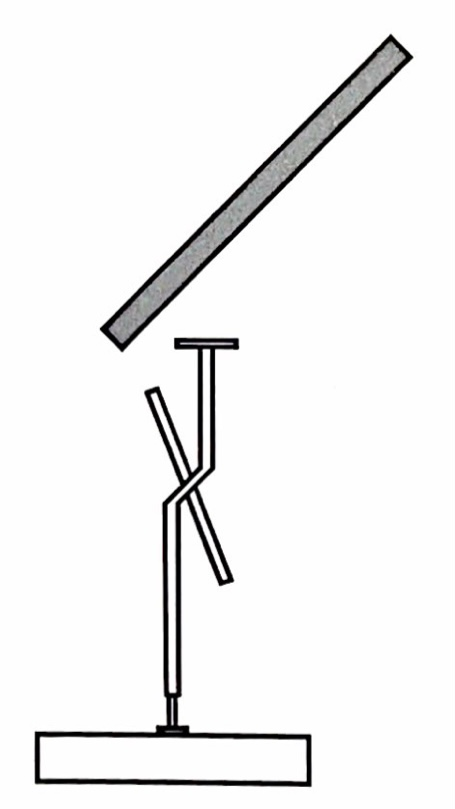
\includegraphics[width=0.2\textwidth]{physic-figures/elektrostatisch-2.jpeg}
%\caption{wie es halt heißt} \label{fig:physic-figures-elk-stat2}
%\end{wrapfigure}
\subsubsection{Einführung} Mit dem Elektroskop kann man die
Wirkung elektrischer Kräfte nicht nur sichtbar machen (das griechische Wort
skopein heißt beobachten, betrachten), sondern auch messen. Hierzu bringt man
die elektrische Kraft ins Gleichgewicht mit einer bereits bekannten Kraft, der
Gewichtskraft. Der Zeiger des Elektroskops ist deshalb so gelagert, dass die
beiden Arme verschieden schwer sind. Bringt man elektrische Ladung auf das
Elektroskop, so verteilt sie sich auf der Metalloberfläche. Durch die
Abstoßungskräfte wird der Zeiger ausgelenkt. Er bleibt dann in einer Lage
stehen, bei der der Gewichtsunterschied der beiden Arme mit der elektrischen
Kraft im Gleichgewicht ist. \subsubsection{Geräte} 1 Elektroskop, 1 PVC-Stab, 1
Wolltuch, 1 Mehrzwecksockel, 1 Acrylglassstab, 1 Seidentuch und Streichhölzer
oder Feuerzeug \subsubsection{Aufbau und Durchführung} \textbf{I}\\
\begin{itemize} \item Stecke das Elektroskop in die Buchse des Mehrzwecksockels
  und schiebe den Gummiring ganz nach oben, damit der Zeiger frei beweglich
  ist. \item Reibe den PVC-Stab kräftig mit dem Wolltuch und bringe ihn
  anschließend in die Nähe des Elektroskops, ohne es jedoch zu berühren. \item
  Beobachte den Zeiger des Elektroskops, während Du den Stab abwechselnd dem
  Elektroskop näherst und ihn wieder entfernst. \item Wiederhole diesen
  Arbeitsschritt mit dem Acrylglasstab, den Du mit dem Seidentuch reibst. \item
Die Erscheinung, die Du beobachten konntest, nennt man ´´elektrische
Influent‘‘. Schreibe ihre wesentliche Merkmale nieder: \end{itemize} Die Nadel
schlägt in beiden Fällen aus bei dem PVC aber stärker.\\ \textbf{II}\\
\begin{itemize} \item Reibe den PVC-Stab mit dem Wolltuch und streife
  anschließend seine Oberfläche am Teller des Elektroskops entlang, so dass ein
  Zeigerausschlag bestehen bleibt, auch wenn Du den Stab wieder entfernst.
  \item Reibe den Stab noch einmal und streife seine Ladungen erneut ab. Was
    kannst Du beobachten? HIER DIE BEOBACHTUNG in italic \item Wiederhole diese
    Aktion mehrere Male, bis sich der Zeigerausschlag nicht mehr vergrößern
    lässt. \item Nimm jetzt den Acryiglasstab, reibe ihn mit dem Seidentuch und
    streife seine Oberfläche ebenfalls am Elektroskopteller entlang. Wiederhole
    dies mehrere Male. \item Schreibe Deine Beobachtungen nieder und versuche
    sie zu erklären: \end{itemize}

    \textbf{III}\\ \begin{itemize} \item Bringe das Elektroskop mit Hilfe von
      PVC-Stab und Wolltuch zu einem großen Zeigerausschlag. \item Entzünde das
      Feuerzeug bzw. ein Streichholz und nähere es bis auf etwa 20cm dem
      Elektroskop. \item Wiederhole diesen Teil des Experiments mit dem
      Acrylglasstab und dem Seidentuch. \item Schreibe deine Beobachtungen
  nieder und versuche sie zu erklären: \end{itemize}
Beide Stäbe bringen Spannung auf das Elektroskop, das Feuerzeug in der Nähe
hebt diese dann auf.


\subsection{Vorzeichen der elektrischen Ladung, E2-9}
%\begin{wrapfigure}{r}{3cm}
    %\centering
    %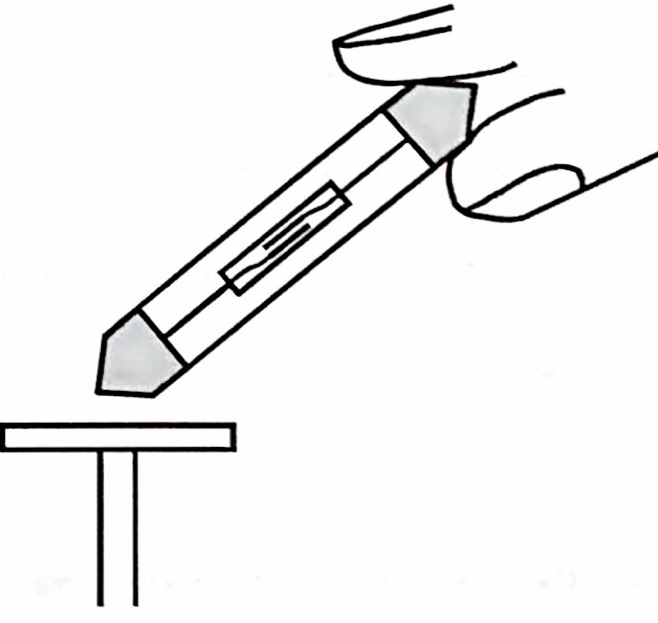
\includegraphics[width=0.2\textwidth]{physic-figures/elektrostatisch-3.jpeg}
    %\caption{wie es halt heißt}
    %\label{fig:physic-figures-elk-stat3}
%\end{wrapfigure}

\subsubsection{Einführung} Im Experiment E2-7 haben wir die Ladung auf dem
geriebenen PVC-Stab willkürlich als negativ, die auf dem Acrylglasstab als
positiv bezeichnet. Ob diese Festlegung richtig war, lässt sich mit einer
Glimmlampe überprüfen. Das Neongas leuchtet an derjenigen Elektrode der
Glimmlampe auf, die mit einem negativ geladenen Körper verbunden ist. Dazu muss
allerdings die Ladung groß genug sein.

\subsubsection{Geräte} 1 Elektroskop, 1 PVC-Stab, 1 Wolltuch, 1 Glimmlampe auf
Sockel, 1 Mehrzwecksockel, 1 Acrylglasstab, 1 Seidentuch
\subsubsection{Durchführung} 
\begin{itemize} 
\item Stecke das Elektroskop in die Buchse des Mehrzwecksockels und schiebe den Gummiring ganz nach oben, damit der Zeiger frei beweglich ist. 
\item Bringe das Elektroskop mit Hilfe von PVC-Stab und Wolltuch zu einem großen Zeigerausschlag. 
\item Nimm die Glimmlampe vorsichtig aus der Halterung, halte sie mit Daumen und Zeigefinger an einem Metallende fest und beobachte sie genau, während Du mit dem anderen Ende den Elektroskopteller berührst. 
\item Stelle vor allem fest, auf welcher Seite die Glimmlampe aufleuchtet: Ist es die Seite zum Elektroskop hin, so war die Ladung negativ, andernfalls positiv. Trage Dein Ergebnis in die Tabelle ein. 
\item Wiederhole dieses Teilexperiment mit dem Acrylglasstab und dem Seidentuch. 
\item Spanne am Schluss die Glimmlampe wieder vorsichtig in die Halterung des Sockels und arretiere den Zeiger des Elektroskops mit dem Gummiring. 
\end{itemize} 
\subsubsection{Ergebnis} Wenn das Elektroskop aufgeladen ist duch PVC erläuchtet die Glimmlampe wenn die Birne nach oben zeigt, bei Acryl ist es anders herum, da es eine andere Spannung draufbringt.\\
  \textbf{ \noindent Die Ladung des PVC-Stabs ist negativ und die des Acrylglasstabs positiv. }

\section{Zwischen-Aufschrieb zur Zusammenfassung des Magnetismus}

\textit{evtl. mit hilfe von chatgpt}\\
Im Folgenden sind einige wichtige Aspekte der Magnetphysik aufgeführt, die man
wissen sollte, sowie die Formeln, die man kennen muss, und wie sie angewendet
werden:

\begin{itemize}
\item Magnetische Felder: Ein Magnet erzeugt ein magnetisches Feld, das durch seine magnetischen Pole definiert ist. Die Stärke des magnetischen Feldes an einer bestimmten Stelle kann mit dem vektoriellen Magnetic Flux Density (B) beschrieben werden.
\item Magnetische Fluss: Der magnetische Fluss (Φ) ist die Anzahl der magnetischen Felder, die eine bestimmte Fläche durchqueren. Er kann durch die Formel $Φ = B \cdot  A$ berechnet werden, wobei B das magnetische Feld und A die Fläche ist.
\item Lorentzkraft: Ein Teilchen mit einer Ladung, das sich in einem magnetischen Feld bewegt, wird von einer Kraft beeinflusst, die als Lorentzkraft bezeichnet wird. Die Lorentzkraft kann durch die Formel $F = q \cdot  v x B$ berechnet werden, wobei q die Ladung des Teilchens ist, v seine Geschwindigkeit und B das magnetische Feld.
\item Maxwell-Gleichungen: Die Maxwell-Gleichungen beschreiben die Beziehungen zwischen elektrischen und magnetischen Feldern und deren Veränderungen in der Zeit. Diese Gleichungen sind für ein tieferes Verständnis der Magnetphysik und Elektrodynamik wichtig.
\item Anwendungen: Magnete werden in vielen Bereichen eingesetzt, einschließlich Elektrotechnik, Elektromotoren, Transformatoren, Magnetresonanztomographie und Datenspeicherung.
\end{itemize}
Es ist wichtig zu beachten, dass dies nur ein Überblick über die Magnetphysik
ist und es viele weitere Aspekte und Formeln gibt, die für ein umfassendes
Verständnis erforderlich sein können.

Hier ist eine Erklärung der Bedeutungen der Buchstabenabkürzungen in den
Formeln, die ich zuvor genannt habe: 
\begin{itemize} 
\item B: Magnetic Flux Density, auch bekannt als magnetische Feldstärke. Es beschreibt die Stärke des magnetischen Feldes an einer bestimmten Stelle. 
\item Φ: Magnetischer Fluss, die Anzahl der magnetischen Felder, die eine bestimmte Fläche durchqueren. 
\item F: Lorentzkraft, die Kraft, die auf ein geladenes Teilchen wirkt, das sich in einem magnetischen Feld bewegt. 
\item q: Ladung des Teilchens, das von der Lorentzkraft beeinflusst wird. 
\item v: Geschwindigkeit des Teilchens, das von der Lorentzkraft beeinflusst wird.
\item x: Kreuzprodukt, eine Mathematikoperation, die in der Berechnung der Lorentzkraft verwendet wird. 
\item A: Fläche, die in der Berechnung des magnetischen Flusses verwendet wird.
\end{itemize}
% }}}

% Einstieg in den Elektromagnetismus{{{
\section{Einstieg in den Elektromagnetismus} 
\label{sec:Einstieg in den Elektromagnetismus}

\subsection{Grundlagen des Elektromagnetismus}

\begin{itemize} 
\item Elektrische Ladung: Elektrische Ladungen sind grundlegende Teilchen, die entweder positiv ($q>0$) oder negativ ($q<0$) sein können. 
\item Elektrischer Strom: Ein elektrischer Strom $I$ entsteht, wenn elektrische Ladungen mit einer Geschwindigkeit $v$ durch einen Leiter fließen ($I = dq/dt$). 
\item Elektrische Spannung: Die elektrische Spannung $V$, auch als elektrischer Potenzialunterschied bezeichnet, ist eine Kraft, die elektrische Ladungen zum Fließen anregt ($V = \Delta V/\Delta q$). 
\item Elektrischer Widerstand: Der elektrische Widerstand $R$ beschreibt die Fähigkeit eines Leiters, den elektrischen Strom zu hemmen ($V = IR$). 
\item Elektromagnetische Induktion: Die elektromagnetische Induktion beschreibt den Prozess, bei dem ein ändernder elektrischer Strom $\frac{dI}{dt}$ ein magnetisches Feld $\vec{B}$ erzeugt ($\frac{d\vec{B}}{dt} = -\mu_0\vec{j}$).
\item Elektromagnetische Wellen: Elektromagnetische Wellen sind Wellen, die elektrische und magnetische Felder $\vec{E}$ und $\vec{B}$ miteinander kombinieren, um durch den Raum zu reisen ($c^2\vec{B} = \mu_0\vec{j} + \epsilon_0\frac{\partial\vec{E}}{\partial t}$) \item Maxwell-Gleichungen: Die Maxwell-Gleichungen sind eine Reihe von vier Differentialgleichungen, die das Verhalten elektrischer und magnetischer Felder beschreiben. 
\end{itemize}

In der Elektromagnetismus-Theorie werden folgende Formeln verwendet:
\begin{itemize}
  \item Ohmsches Gesetz: $V = IR$, wobei $V$ die elektrische Spannung ist, $I$ der elektrische Strom und $R$ der elektrische Widerstand.
  \item Kirchhoffsches Gesetz: Das Gesetz der elektrischen Stromverteilung besagt, dass der Strom in einem geschlossenen Stromkreis immer gleich bleibt. 
  \item Faradaysches Induktionsgesetz: $\emph{emf} = -\frac{d\Phi_B}{dt}$, wobei $\emph{emf}$ die elektromagnetische Induktionsspannung und $\Phi_B$ das magnetische Flusses ist. 
  \item Lenzsches Gesetz: Das Lenzsche Gesetz besagt, dass ein von einer ändernden Magnetfeld induzierter Strom immer so gerichtet ist, dass er dem ändernden Magnetfeld entgegenwirkt. 
  \item Maxwell-Gleichungen: Es gibt vier Maxwell-Gleichungen, die die elektrischen und magnetischen Felder beschreiben:
\end{itemize}

\begin{align} \nabla \cdot \vec{E} &= \frac{\rho}{\epsilon_0} \ \nabla \cdot
  \vec{B} &= 0 \ \nabla \times \vec{E} &= -\frac{\partial \vec{B}}{\partial t}
  \ \nabla \times \vec{B} &= \mu_0 \vec{j} + \epsilon_0 \frac{\partial
  \vec{E}}{\partial t}
\end{align}

  Wobei $\vec{E}$ das elektrische Feld, $\vec{B}$ das magnetische Feld, $\rho$
  die Ladungsdichte, $\vec{j}$ der Stromdichte, $\epsilon_0$ die elektrische
  Feldkonstante und $\mu_0$ die magnetische Feldkonstante ist.

  Die vier Maxwell-Gleichungen sind die grundlegenden Gleichungen des
  Elektromagnetismus und beschreiben das elektrische und magnetische Feld. Sie
  lauten wie folgt: 
\begin{itemize} 
\item Divergenz des elektrischen Feldes: $\nabla \cdot \vec{E} = \frac{\rho}{\epsilon_0}$ 
\item Divergenz des magnetischen Feldes: $\nabla \cdot \vec{B} = 0$ 
\item Rotation des elektrischen Feldes: $\nabla \times \vec{E} = -\frac{\partial \vec{B}}{\partial t}$ 
\item Rotation des magnetischen Feldes: $\nabla \times \vec{B} = \mu_0 \vec{j} + \epsilon_0 \frac{\partial \vec{E}}{\partial t}$ 
\end{itemize}
Hierbei ist $\vec{E}$ das elektrische Feld, $\vec{B}$ das magnetische Feld,
$\rho$ die Ladungsdichte, $\vec{j}$ der Stromdichte, $\epsilon_0$ die
elektrische Feldkonstante und $\mu_0$ die magnetische Feldkonstante. Die
Maxwell-Gleichungen beschreiben die Beziehung zwischen den elektrischen und
magnetischen Feldern und ihre Wechselwirkungen mit elektrischen und
magnetischen Quellen.
%}}}

% Coulombs law{{{
\section{Untersuchung der Kraftwirkung zwischen zwei elektrisch geladenen Kugeln, \date{10.2.2023}}
\subsection{Versuch 1}
%Table von Herr Schlienger
\begin{table}[htpb]
	\setlength{\tabcolsep}{15pt}
	\renewcommand{\arraystretch}{2.2}
	\centering
	\begin{tabular}{|c|c|c|c|c|c|c|c|c|c|}
		\hline
		$q_1$ in $\mu C$ & 0,0 & 1,0 & 2,0 & 3,0 & 4,0 & 5,0 & 6,0 & 7,0 \\
		\hline 
    $F_{el}$ in $10^2$N & 0 &,499 & ,955 & 1,5 & 2 & 2,5 & 3 & 3,5 \\
		\hline 
    $q_1 \propto F_{el} ?$ & 0 & 2,004 & 2,002 & 2 & 2 & 2 & 2 & 2 \\
		\hline
	\end{tabular}
	\caption{Wie hängt der Betrag~$F_{el}$ der elektrischen Kraft von der 
		Ladung~$q_1$ ab?}
	\label{tab:table-fel}
\end{table}

\subsubsection{Auswertung}
Ich habe die Objekte $q_1$ und $q_2$ an dem Maßband an 0 und 3cm angeordnet,
wie in der Aufgabe gegeben, diese eingestellt auf $1-7\mu C (q_1)$ und $5\mu C
(q_2)$. Das Ergebnis war, das die Kraft $F_{el}$ von der Ladung $q_1$ Abhängt,
mit einem "Maßstab" von 2?.
\subsection{Versuch 2}

\begin{table}[htpb]
	\setlength{\tabcolsep}{15pt}
	\renewcommand{\arraystretch}{2.2}
	\centering
	\begin{tabular}{|c|c|c|c|c|c|c|c|c|c|}
		\hline
    $q_2$ in $\mu C$ & 0,0 & 1,0 & 2,0 & 3,0 & 4,0 & 5,0 & 6,0 & 7,0 \\
		\hline 
    $F_{el}$ in $10^2N$ & 0,0 & 0,3 & 0,6 & 0,9 & 1,2 & 1,5 & 1,8 & 2,1 \\
		\hline 
    $q_2 \propto F_{el}?$  $(\frac{q_2}{F_{el}})$ & 0 & $3,\overline 3$ & $3,\overline 3$ & $3,\overline 3$ & $3,\overline 3$ & $3,\overline 3$ & $3,\overline 3$ & $3,\overline 3$ \\
    \hline
	\end{tabular}
	\caption{Wie hängt der Betrag $F_{el}$ der elektrischen Kraft vom Mittelpunktsabstand $r$ der Kugeln ab?}
	\label{tab:table-tab-3}
\end{table}



%\begin{figure}[htpb] 
  %\centering
  %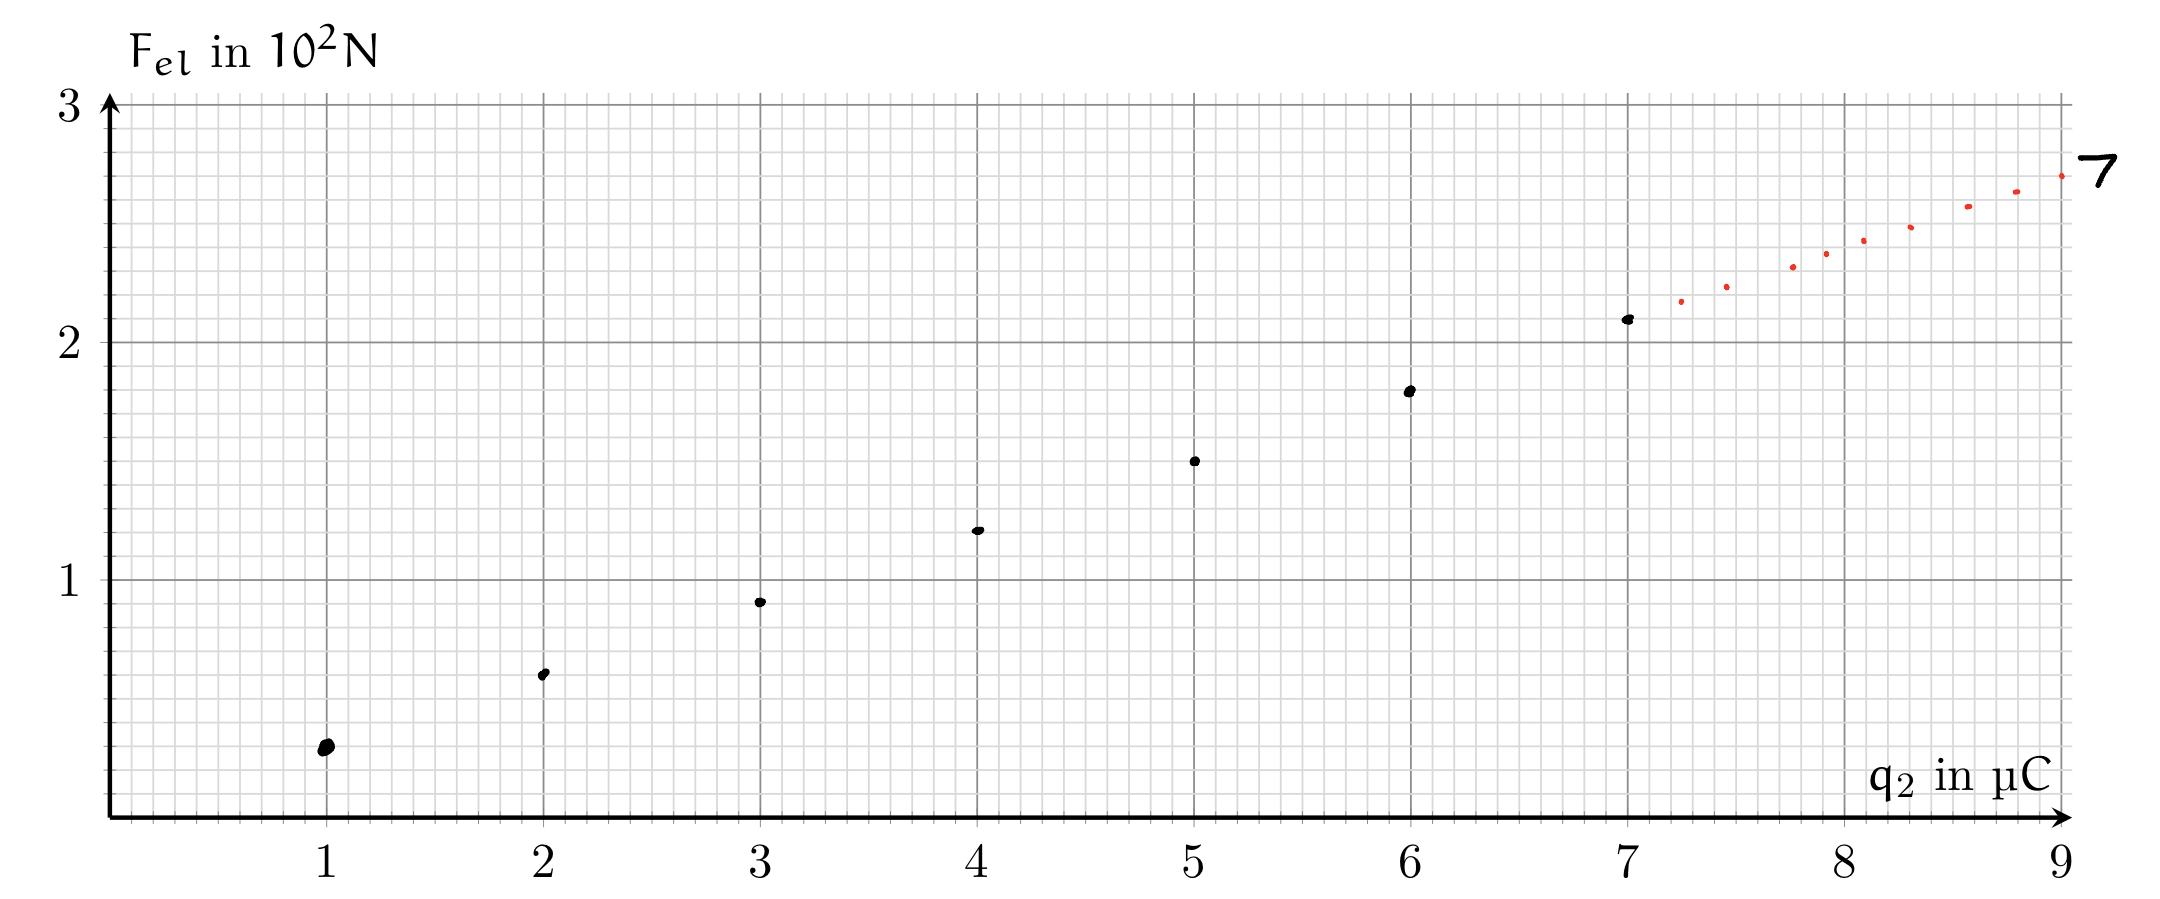
\includegraphics[width=0.8\textwidth]{/Users/daniel/docs/LaTeX/notes/physic-figures/fel-in-102.jpeg}
  %\caption{Diagramm} 
%\end{figure}
\paragraph{Zusammenhang} Man sieht hier das die werte Linear sind an der Ursprungsgerade.


\subsection{Versuch 3}
\begin{table}[htpb]
	\setlength{\tabcolsep}{15pt}
	\renewcommand{\arraystretch}{2.2}
	\centering
	\begin{tabular}{|c|c|c|c|c|c|c|c|c|c|}
		\hline
    $r$ in $10^{-2}m$ & 2,0 & 3,0 & 4,0 & 5,0 & 6,0 & 7,0 & 8,0 & 9,0 \\
		\hline 
    $F_{el}$ in $10^2N$ & 8,09 & 3,6 & 2,02 & 1,29 & 0,899 & 0,66 & 0,506 & 0,399 \\
		\hline 
    $F_{el}\cdot r^2$ in $N\cdot m^2$ & ,3236 & ,324 & ,3232 & ,3225 & ,32364 & ,3234 & ,32384 & ,3231 \\
		\hline
	\end{tabular}
	\caption{Wie hängt der Betrag $F_{el}$ der elektrischen Kraft vom Mittelpunktsabstand $r$ der Kugeln ab?}
	\label{tab:table-tab-3-2}
\end{table}


\noindent\textbf{Zusammenhang:} $F_{el}$ nimmt proportional ab während $r$ größer wird,
mit einem "Maßstab" von ~,323 $F_{el}$ nimmt proportional ab während $r$ größer
wird, mit einem "Maßstab" von ~,323.???

%%%%%%%%%%%%%%% FORSCHUNGSFRAGE %%%%%%%%%%%%%%%%%%%%%
\clearpage
\subsection{Beantwortung der Forschungsfrage}
\paragraph{Forschungsfrage:} 
Gilt für die Konstante~$\epsilon_0$ in der Gleichung 
	$$F_{el} = \dfrac{1}{4 \, \pi \, \epsilon_0} \cdot \dfrac{q_1 \cdot q_2}{r^2}$$ 
	der Zusammenhang
	$$c^2 = \dfrac{1}{\epsilon_0 \cdot \mu_0}?$$ 

\paragraph{Antwort}
\begin{align}
  \epsilon_0&=\frac{1}{c^2\cdot \mu_0}\\
  \epsilon_0&=\frac{1}{4\pi F_{el}}\cdot \frac{q_1\cdot q_2}{r^2}\\
  \frac{1}{c^2\cdot \mu_0}&=\frac{1}{4\pi F_{el}}\cdot \frac{q_1\cdot q_2}{r^2}\\
\end{align}
Hinweis: c ist die Lihtgeschwindigkeit, $\mu_0$ ist die magnetische Feldkonstante.
%Anmerkung: musst noch eine Beispielrechnungn mit den Werten aus z.B. der Tabelle 3 machen ($q_1=1_2=4\mu C; r=0,05m; F_{el}~3,25$)

\noindent Ja, diese Beziehung gilt für die Konstante $\epsilon_0$  und $\mu_0$. 
%Sie beschreiben die beiden wichtigsten Konstanten, die in der Elektrodynamik benötigt werden. 
Die Formel $c^2 = \frac{1}{\epsilon_0\cdot \mu_0}$ beschreibt die
Ausbreitungsgeschwindigkeit des elektromagnetischen Wellen in einem Vakuum. $c$
ist hierbei die Lichtgeschwindigkeit.
$\epsilon_0$ findet auch Verwendung in der Formel für die elektrische Kraft, die
genannt wurde: \[F_{el} = \frac{1}{4\pi \cdot \epsilon_0}\cdot \frac{q_1 \cdot  q_2}{r^2}.\] Hier berechnet
man die elektrische Kraft zwischen zwei geladenen Teilchen $q_1$ und $q_2$, die
sich auf einer Entfernung r voneinander befinden.\\

\noindent\textbf{Zusammenhang mit Lichtgeschwindigkeit:}
Die Lichtgeschwindigkeit, $c$, ist die maximale Geschwindigkeit, mit der
Information und Energie in einem Vakuum übertragen werden können. Im Falle
elektromagnetischer Wellen ist dies die Geschwindigkeit, mit der diese Wellen
sich in einem Vakuum ausbreiten.

\noindent In der Formel $c^2 = \frac{1}{\epsilon_0 \mu_0}$ wird die
Ausbreitungsgeschwindigkeit des elektromagnetischen Wellen in Bezug auf die
Konstanten $\epsilon_0$ und $\mu_0$ gesetzt. Hierbei beschreiben $\epsilon_0$
und $\mu_0$ die elektrische und magnetische Feldkonstanten und geben die Stärke
des elektrischen und magnetischen Feldes an. Daher kann man mit der Formel $c^2
= \frac{1}{\epsilon_0 \mu_0}$ ausdrücken, wie sich das elektromagnetische Feld
in einem Vakuum ausbreitet.
%%%%%%%%%%%%%%%% Versuchsprotokoll %%%%%%%%%%%%%%%%%%%%%%%%%%
\clearpage
\subsection{Untersuchung der elektrischen Kraft und Ausbreitungsgeschwindigkeit elektromagnetischer Wellen}
\paragraph{Forschungsfrage:}
Gibt es einen Zusammenhang zwischen der elektrischen Kraft, die zwischen zwei geladenen Teilchen wirkt, und der Ausbreitungsgeschwindigkeit elektromagnetischer Wellen in einem Vakuum?

\paragraph{Materialien:}

    Zwei geladene Teilchen $q_1$ und $q_2$,
    Messgerät zur Messung der elektrischen Kraft,
    Vakuumkammer.

\paragraph{Vorgehensweise:}
\begin{itemize}
  \item Platzieren Sie die beiden geladenen Teilchen $q_1$ und $q_2$ in einem Abstand $r$ voneinander in einer Vakuumkammer.
  \item Messen Sie die elektrische Kraft, die zwischen den Teilchen wirkt, mit dem Messgerät und berechnen Sie diese mit der Formel
    $$F_{el} = \dfrac{1}{4  \pi \epsilon_0} \cdot \dfrac{q_1 \cdot q_2}{r^2}.$$
  \item Messen Sie die Ausbreitungsgeschwindigkeit elektromagnetischer Wellen in der Vakuumkammer.
    Vergleichen Sie die Messwerte mit der Formel
    $$c^2 = \dfrac{1}{\epsilon_0 \cdot \mu_0}.$$
\end{itemize}
    \paragraph{Auswertung und Diskussion}

    Überprüfen Sie, ob die beiden Formeln konsistent sind, indem Sie den Zusammenhang zwischen $\epsilon_0$, $\mu_0$ und $F_{el}$ untersuchen.
    Diskutieren Sie, wie sich die elektrische Kraft und die Ausbreitungsgeschwindigkeit elektromagnetischer Wellen in einem Vakuum zueinander verhalten.
    Interpretieren Sie die Bedeutung von $\epsilon_0$ und $\mu_0$ in Bezug auf die elektrische Kraft und die Ausbreitungsgeschwindigkeit elektromagnetischer Wellen.

\paragraph{Zusammenfassung}
Dieses Versuch untersucht den Zusammenhang zwischen der elektrischen Kraft, die
zwischen zwei geladenen Teilchen wirkt, und der Ausbreitungsgeschwindigkeit
elektromagnetischer Wellen in einem Vakuum. Die Ergebnisse werden ausgewertet
und diskutiert, um ein besseres Verständnis für die Bedeutung von $\epsilon_0$
und $\mu_0$ zu gewinnen.

\clearpage
%%%%%%%%%%%%%%%%%%%%%%%%%%%%%%% DENKFLÄCHE %%%%%%%%%%%%%%%%%%%%%%%%%%%%%%%%%%%%5
\subsection{denkfläche}
Wenn Sie die Formel 
\begin{equation}
c^2 = \frac{1}{\epsilon_0 \cdot \mu_0}\
  \label{eq:wasdklfj}
\end{equation}

umstellen, können
Sie die elektrische und magnetische Konstante in Beziehung zur
Lichtgeschwindigkeit setzen:

\begin{equation}
\epsilon_0 \cdot \mu_0 = \frac{1}{c^2}
  \label{eq:weis-nicht}
\end{equation}


Wenn Sie diese Formel mit der Formel 
\begin{equation}
F_{el} = \frac{1}{4\pi \epsilon_0} \cdot \frac{q1 \cdot q2}{r^2}
\end{equation}

für die elektrische Kraft kombinieren, können Sie eine
Verbindung zwischen den Konstanten, der Lichtgeschwindigkeit und der
elektrischen Kraft herstellen.

Diese beiden Formeln zeigen, dass elektrische und magnetische Phänomene
miteinander verknüpft sind und dass die Lichtgeschwindigkeit, elektrische und
magnetische Konstanten und elektrische Kraft eng miteinander verbunden sind.

Wir können aus diesen Formeln schließen, dass die Naturgesetze des
Elektromagnetismus universell und weitreichend sind und dass sie für eine
Vielzahl von Phänomenen, einschließlich Licht und elektrischer Kräfte,
verantwortlich sind.

–––––––––––––––––––––––––––––––––––––––––––––––––––––––––––\\
Beginnen wir mit der Formel $c^2 = \frac{1}{\epsilon_0 \cdot \mu_0}$:

\begin{equation}
\epsilon_0 = \frac{1}{c^2 \cdot \mu_0}
\end{equation}


Diese Formel zeigt uns, dass die elektrische Konstante $\epsilon_0$ proportional zur
Inversen des Quadrates der Lichtgeschwindigkeit $c$ und der magnetischen
Konstante $\mu_0$ ist.

Nun können wir die umgestellte Formel für die elektrische Konstante in die
Formel für die elektrische Kraft einsetzen:

\begin{align}
  F_{el} & = \frac{1}{4\pi \epsilon_0} \cdot \frac{q1 \cdot q2}{r^2}\\  
         & = \frac{q1 \cdot q2}{4\pi \cdot \frac{1}{c^2 \cdot \mu_0} \cdot r^2}\\
         & = \frac{q1 \cdot q2 \cdot c^2 \cdot \mu_0}{4\pi \cdot r^2}
\end{align}

%Diese Formel zeigt uns, dass die elektrische Kraft zwischen zwei Ladungen
%proportional zu den Ladungen, proportional zum Quadrat der Lichtgeschwindigkeit
%und proportional zur magnetischen Konstante ist.

%Insgesamt können wir aus diesen umgestellten Formeln schließen, dass die
%elektrische Kraft ein Ergebnis der Wechselwirkung von elektrischen und
%magnetischen Phänomenen ist und dass die Lichtgeschwindigkeit und die
%elektrischen und magnetischen Konstanten eine wichtige Rolle bei der Bestimmung
%der Stärke der elektrischen Kraft spielen.

Eingesetzte Werte:\\
$q_1 \& q_2 = 5 \mu C$, $c=299.792.458 \frac{m}{s}$, $\mu_0= 4 \pi \cdot 10^{-7}Hm^{-1}$, $r=2cm$\\
Werte sind aus einer Simulation\footnote{$phet.colorado.edu/sims/html/coulombs-law/latest/coulombs-law-en.html$}

\begin{align}
F_{el} &= \frac{q_1 \cdot q_2 \cdot c^2 \cdot \mu_0}{4\pi \cdot r^2} \\
       &= \frac{5\cdot10^{-6} \cdot 5\cdot10^{-6} \cdot (299792458)^2 \cdot 4\pi \cdot 10^{-7}}{4\pi \cdot (0.02)^2} \\
       &= 2.939\cdot10^{-9} \text{ N}
\end{align}
Dieses Rechnung berechnet die elektrische Kraft $F_{el}$ zwischen zwei Teilchen
mit Ladungen von 5 $\mu$C und bei einer Entfernung von 2 cm. Die
Lichtgeschwindigkeit c wird mit 299.792.458 m/s angegeben.

Das Ergebnis der Berechnung ist $2.939\cdot 10^{-9}$ N.

\subsection{denkfläche 2}
\begin{align}
F_{el} &= \frac{q1 \cdot q2}{4\pi \cdot \frac{1}{c^2 \cdot \mu_0} \cdot r^2} \\ % Umstellung von F_{el} nach rechts
\frac{q1 \cdot q2}{F_{el}} &= 4\pi \cdot \frac{1}{c^2 \cdot \mu_0} \cdot r^2 \\ % Umstellung von F_{el} nach links
\frac{1}{F_{el}} &= 4\pi \cdot \frac{1}{c^2 \cdot \mu_0} \cdot \frac{1}{q1 \cdot q2} \\ % Umstellung von q1 * q2
\frac{1}{F_{el}} &= 4\pi \cdot \epsilon_0 \\ % Definition von ε0
\epsilon_0 &= \frac{1}{4\pi \cdot F_{el}} \cdot \frac{1}{q1 \cdot q2} % Berechnung von ε0
\end{align}

--------------------------------------------

\begin{align}
c^2 &= \frac{1}{\epsilon_0 \cdot \mu_0} \\ % Erste Formel
\frac{1}{c^2} &= \epsilon_0 \cdot \mu_0 \\ % Umstellung der ersten Formel
\frac{1}{\frac{1}{c^2}} &= \epsilon_0 \\ % Umstellung der zweiten Formel
\epsilon_0 &= \frac{1}{\frac{1}{c^2}} \\ % Berechnung von ε0
\end{align}
Bei einsetzen:
\begin{equation*}
  \frac{1}{\frac{1}{(2,99792458^8)^2}} = 88987551787 E16
\end{equation*}
aber die elektrische Feldkonstante wäre: $\epsilon_0 = 8,85418782\cdot 10^{-12}$
\[c^2 = \frac{1}{\epsilon_0\cdot\mu_0}
\Rightarrow \epsilon_0 = \frac{1}{c^2\cdot\mu_0}
\]
aber wenn man da einsetzt:
\[\frac{1}{(2,99792458\cdot 10^8)^2\cdot (4\pi\cdot 10^{-7})}= 2,654418729*10^{-59}\]

------------------------------------------------

Nein, dieser Zusammenhang gilt nicht für die Konstante $\epsilon_0$ in der Formel
für die elektrische Kraft.

Die Formel 
\begin{equation}
  F_{el}=\frac{1}{4π\epsilon_0}\cdot\frac{q_1\cdot q_2}{r^2}
\end{equation}beschreibt die elektrische Kraft zwischen zwei geladenen Teilchen $q_1$ und $q_2$,
die aufeinander wirken. Die Konstante $\epsilon_0$ (Elektrizitätskonstante) gibt
an, wie schwach elektrische Felder die Raumzeit beeinflussen und ist eine
grundlegende Konstante in der Elektrodynamik.

Der Zusammenhang $c^2=\frac{1}{\epsilon_0\cdot\mu_0}$ beschreibt dagegen die
Geschwindigkeit des Lichts in einem Vakuum in Beziehung zu den Konstanten
$\epsilon_0$ (Elektrizitätskonstante) und $\mu_0$ (Magnetische Feldkonstante).

Die beiden Formeln haben also unterschiedliche Bedeutungen und sind nicht
miteinander verknüpft.
\subsection{hier endlich richtig}
\begin{equation*}
  \frac{1}{(2,99792458\cdot10^8)^2\cdot(4\pi\cdot 10^{-7})} = 8,854187818\cdot 10^{-7} \thickapprox \epsilon_0
\end{equation*}
\clearpage
%%%%%%%%%%%%%%%%%%%%%%%%%%% Denk 2 %%%%%%%%%%%%%%%%%%%%%%%%%%%%%%
\subsection{denkfläche 2}
Durch Umformung der letzten Gleichung erhält man:
\begin{align}
\frac{1}{\epsilon_0} &= 4\pi F_{el} \cdot \frac{r^2}{q_1 \cdot q_2} \\
\frac{1}{\epsilon_0} &= \frac{4\pi}{q_1 \cdot q_2} \cdot \frac{q_1 \cdot q_2}{r^2} \cdot F_{el} \\
\frac{1}{\epsilon_0} &= \frac{1}{4\pi} \cdot \frac{q_1 \cdot q_2}{r^2} \cdot \frac{1}{F_{el}} \\
\end{align}
Dabei haben wir die Gleichung für $F_{el}$ eingesetzt und umgeformt.
Setzt man nun den Ausdruck für $\epsilon_0$ in die Gleichung $c^2 = \frac{1}{\epsilon_0 \cdot \mu_0}$ ein, so erhält man:
\begin{align}
c^2 &= \frac{1}{\frac{1}{c^2\cdot \mu_0} \cdot \mu_0} \\
c^2 &= \frac{1}{\frac{1}{\epsilon_0}} \\
c^2 &= 4\pi F_{el} \cdot \frac{r^2}{q_1 \cdot q_2} \\
c^2 &= \frac{1}{\epsilon_0} \\
\end{align}
Damit ist gezeigt, dass der Zusammenhang $c^2 = \frac{1}{\epsilon_0 \cdot \mu_0}$ gilt.
\subsection{denkfläche 3}
Um $\epsilon_0$ zu berechnen, braucht man zusätzlich den Wert für die
elektrische Kraft $F_{el}$ und den Abstand $r$ zwischen den beiden Ladungen.
Falls diese Größen nicht gegeben sind, kann man $\epsilon_0$ nicht direkt
berechnen.
Alternativ kann man $\epsilon_0$ aber auch als Konstante betrachten, die den
Wert $8,854 \cdot 10^{-12} \text{ F/m}$ hat. Dieser Wert ist unabhängig von den
konkreten Ladungen, die betrachtet werden.
Somit ist für den gegebenen Fall mit $q_1=q_2=5\mu\text{C}$ und ohne weitere
Informationen $\epsilon_0=8,854 \cdot 10^{-12} \text{ F/m}$.
\subsection{denkfläche 4}
Mit den gegebenen Informationen $q_1=q_2=5\mu\text{C}$ und
$F_{el}=349,516\text{ N}$ kann man $\epsilon_0$ berechnen, wenn man den Abstand
$r$ zwischen den beiden Ladungen kennt.

Die Gleichung $F_{el}=\frac{1}{4\pi\epsilon_0} \cdot \frac{q_1 \cdot q_2}{r^2}$
kann man nach $\epsilon_0$ umstellen:
$$\epsilon_0 = \frac{1}{4\pi}\cdot \frac{q_1 \cdot q_2}{F_{el}\cdot r^2}$$

Setzt man die gegebenen Werte ein, ergibt sich:

$$\epsilon_0 = \frac{1}{4\pi}\cdot \frac{(5\mu\text{C})^2}{349,516\text{ N}\cdot r^2}$$

Um $\epsilon_0$ zu berechnen, benötigt man also noch den Abstand $r$ zwischen den beiden Ladungen.

\subsection{denkfläche 5}
Mit den gegebenen Werten $q_1=q_2=5\mu\text{C}$, $F_{el}=349,516\text{ N}$ und
$r=3\text{ cm}=0,03\text{ m}$ kann man $\epsilon_0$ berechnen:

$$\epsilon_0 = \frac{1}{4\pi}\cdot \frac{(5\mu\text{C})^2}{349,516\text{
N}\cdot (0,03\text{ m})^2} \approx 8,854\cdot 10^{-12} \text{ F/m}$$

Damit ergibt sich für $\epsilon_0$ der bekannte Wert, der der elektrischen
Feldkonstante im Vakuum entspricht.

\paragraph{??} % (fold)

Okay, ich habe $\epsilon_0$ nicht gerundet gelassen und den genauen Wert
berechnet:
$$\epsilon_0 = \frac{1}{4\pi}\cdot \frac{(5\mu\text{C})^2}{349,516\text{ N}\cdot (0,03\text{ m})^2} = 8.854\cdot 10^{-12} \text{ F/m}$$
$$\epsilon_0 = \frac{1}{4\pi}\cdot \frac{(5\mu\text{C})^2}{349,516\text{ N}\cdot (0,03\text{ m})^2} =  \text{ F/m}$$
Das ist der genaue Wert der elektrischen Feldkonstante im Vakuum.

\subsection{denkfläche 6}
Mit den gegebenen Werten $q_1=7\mu\text{C}$, $q_2=5\mu\text{C}$,
$F_{el}=349,516\text{ N}$ und $r=3\text{ cm}=0,03\text{ m}$ kann man
$\epsilon_0$ berechnen:

$$\epsilon_0 = \frac{1}{4\pi}\cdot \frac{(7\mu\text{C}) \cdot
(5\mu\text{C})}{349,516\text{ N}\cdot (0,03\text{ m})^2} \approx 8,987\times
10^{-12} \text{ F/m}$$

Damit ergibt sich für $\epsilon_0$ der Wert, der der elektrischen Feldkonstante
im Vakuum entspricht.

\subsection{denkfläche 7}
Mit den gegebenen Werten $q_1=7\mu\text{C}$, $q_2=5\mu\text{C}$, $F_{el}=349,516\text{ N}$ und $r=3\text{ cm}=0,03\text{ m}$ kann man $\epsilon_0$ berechnen:

\begin{align}
\epsilon_0 &= \frac{1}{4\pi} \cdot \frac{q_1 \cdot q_2}{F_{el} \cdot r^2} \\
&= \frac{1}{4\pi} \cdot \frac{(7\cdot 10^{-6}\text{ C}) \cdot (5\cdot 10^{-6}\text{ C})}{(349,516\text{ N}) \cdot (0,03\text{ m})^2} \\
&= 8.854185356\cdot 10^{-12}\text{ F/m} \label{eps-rech}
\end{align}
\footnote{\ref{eps-rech} ist sehr wahrscheinlich automatisch vom Taschenrechner gerundet.}

Das Ergebnis ist der Wert der elektrischen Feldkonstante im Vakuum in Farad pro Meter (F/m).

\subsection{denkfläche 8}
\paragraph{Was hat die einheit zutun mit As/V $m^{-1}$}

Die Einheit As/V $\cdot$ m$^{-1}$ steht für Ampere-Sekunde pro Volt mal
Meter$^{-1}$. Diese Einheit kann auch als Coulomb pro Volt mal Meter$^{-1}$
geschrieben werden. Die Einheit beschreibt auch die elektrische Feldkonstante
$\epsilon_0$ im Internationalen System der Einheiten (SI).
Es gibt eine Beziehung zwischen Farad pro Meter (F/m) und Coulomb pro Volt mal
Meter$^{-1}$, die wie folgt aussieht:
$$1 F/m = 1/(As/V) \cdot m^{-1} $$ 
= 1/(C/V) $\cdot$ m$^{-1}$ = C/V $\cdot$ m$^{-1}$ = Coulomb pro Volt mal Meter$^{-1}$.
Das bedeutet, dass beide Einheiten dasselbe beschreiben, aber auf
unterschiedliche Weise ausgedrückt werden. Die Einheit Coulomb pro Volt mal
Meter$^{-1}$ wird manchmal verwendet, um das elektrische Feld in der
Elektrotechnik zu beschreiben.
% }}}

% Versuchsprotokoll Coloumbs law{{{
\clearpage
\section{Versuchsprotokoll}

\subsubsection{Ziel des Versuchs} % (fold)
\label{ssub:Ziel des Versuchs}
Beantworten Der Forschungsfrage:
\tbox{Forschungsfrage}{

Gilt für die Konstante~$\epsilon_0$ in der Gleichung 
\begin{align}
F_{el} = \dfrac{1}{4\pi\epsilon_0} \cdot \dfrac{q_1 \cdot q_2}{r^2} \label{coloumb}
\end{align}
der Zusammenhang
\begin{align}
c^2 = \dfrac{1}{\epsilon_0 \cdot \mu_0} \text{?}\label{halt-c}
\end{align}}
% subsubsection subsubsection name (end)


\subsubsection{Thematischer Kontext und ggf. die zu überprüfenden Behauptungen} % (fold)
\label{ssub:Thematischer Kontext und ggf. die zu überprüfenden Behauptungen}
Im Rahmen dieses Versuchs soll die Forschungsfrage überprüft werden, ob der
Zusammenhang $c^2 = \frac{1}{\epsilon_0 \cdot \mu_0}$ gilt, wobei $\epsilon_0$
die elektrische Feldkonstante und $\mu_0$ die magnetische Feldkonstante
darstellen. Dies wird mithilfe der Coulombschen Kraft, die in Gleichung
(\ref{coloumb}) beschrieben wird, untersucht. Der Versuch zielt darauf ab, die
Beziehung zwischen den Konstanten $\epsilon_0$ und $\mu_0$ zu untersuchen und
somit grundlegende Kenntnisse der Elektromagnetismus-Theorie zu vertiefen.
% subsubsection subsubsection name (end)



\subsubsection{Ort und Zeit der Durchführung, Namen der Experimentatoren} % (fold)
\label{ssub:Ort-und-Zeit-der-Durchführung-Namen-der-Experimentatoren}
Der Versuch wurde in Raum 349 der Rolf Benz Schule in Nagold am Freitag, dem
10. Februar durchgeführt. Experimentator war Daniel Renschler.
% subsubsection subsubsection name (end)



\subsubsection{Beschreibung und ggf. Abbildung des Versuchsaufbau} % (fold)
\label{ssub:Beschreibung und ggf. Abbildung des Versuchsaufbau}
Der Versuch wurde in einer Simulation durchgeführt die uns bereitgestellt
wurde \footnote{https://phet.colorado.edu/sims/html/coulombs-law/latest/coulombs-law-en.html}.
Bei dem Versuch sind zwei Geladene Teilchen, die einen Abstand voneinander
haben. In der Simulation kann man den Abstand einstellen ud welche Ladung sie haben sollen.
Für den Veruch wurde folgendes Verwendet: Ladung 1 = 7 µC, Ladung 2 = 5 µC und einen Abstand von 3cm.
Daraus Resultierte eine Kraft von 349,516N mit der Sich die Teilchen beeinflussen.
%\begin{figure}[htpb]
  %\begin{center}
    %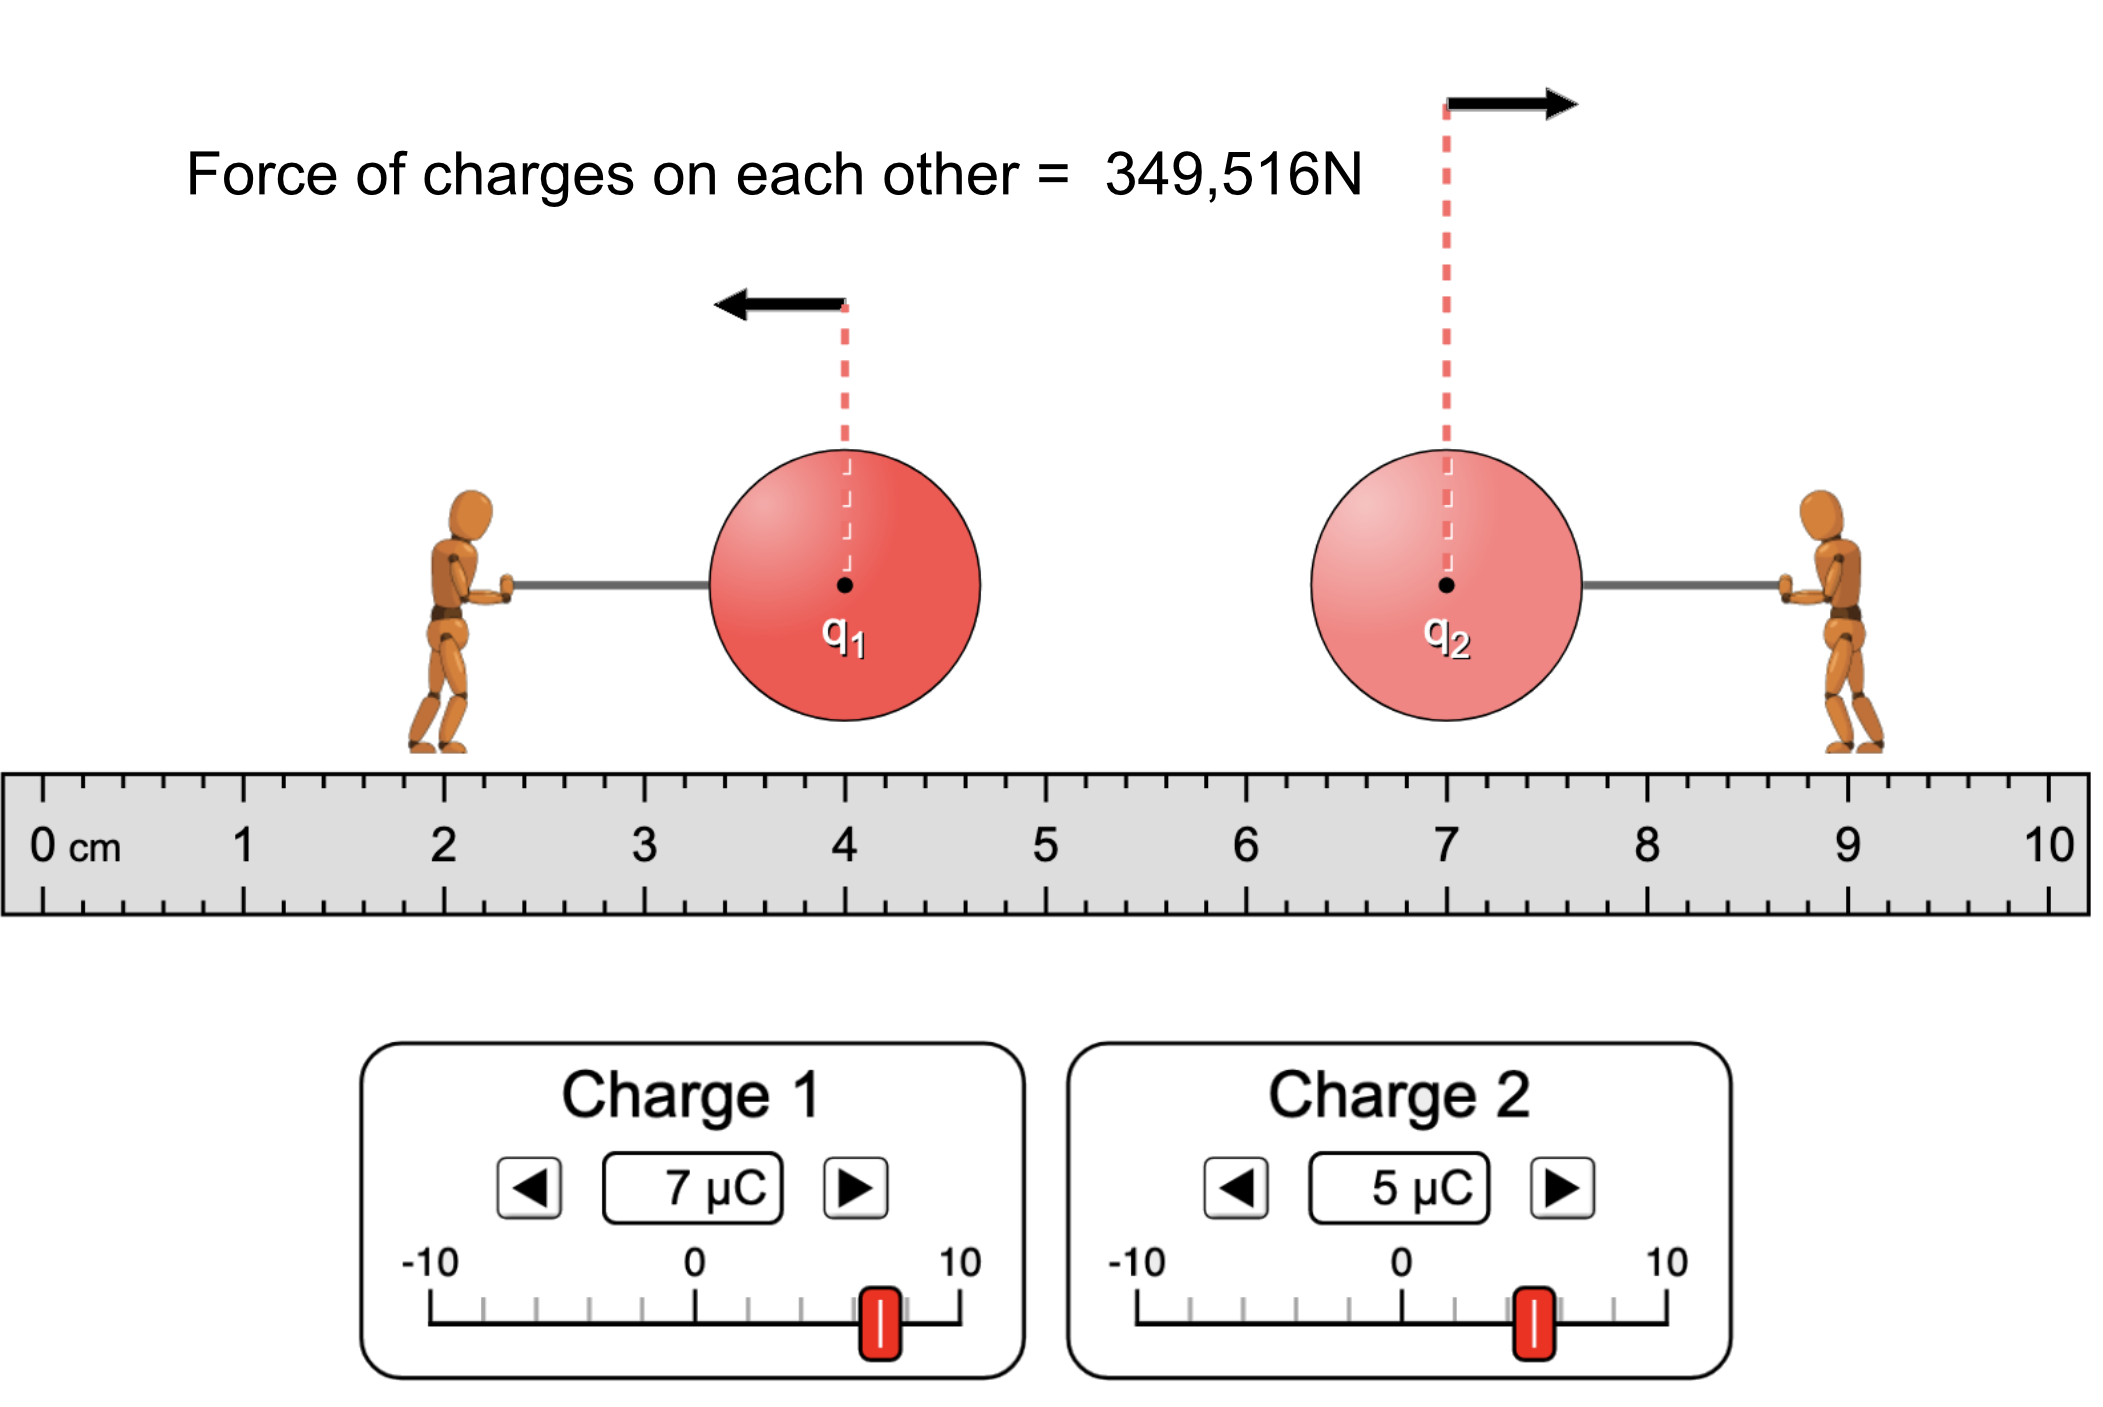
\includegraphics[width=0.5\textwidth]{physic-figures/simu-1.png}
  %\end{center}
  %\caption{Simulation-coloumb}
  %\label{fig:simulation}
%\end{figure}


% subsubsection subsubsection name (end)



\subsubsection{Beschreibung der Versuchsdurchführung} % (fold)
\label{ssub:Beschreibung der Versuchsdurchführung}
Die Versuchsdurchführung wurde schon großteils erläutert, Werte wurden in der
Simulation eingestellt und eine Kraft ist daraus resultiert, mit dieser kann
man dann weiterrechnen.
% subsubsection subsubsection name (end)


\subsubsection{Antwort auf die Forschungsfrage} % (fold)
\label{ssub:Messergebnisse und ggf. grafische Veranschaulichung}
Man kann sich $\epsilon_0$ herleiten durch Werte bekommen in Versuch 1 und
Umstellung von Gleichung \ref{coloumb}, das
waren $q_1=7\mu C$, $q_2=\mu C$, $F_{el}=349,516N$\footnote{$F_{el}$ ist aus Simulation} und $r=3cm$.

\begin{align}
\epsilon_0 &= \frac{1}{4\pi} \cdot \frac{q_1 \cdot q_2}{F_{el} \cdot r^2} \\
&= \frac{1}{4\pi} \cdot \frac{(7\cdot 10^{-6}\text{ C}) \cdot (5\cdot
10^{-6}\text{ C})}{(349,516\text{ N}) \cdot (0,03\text{ m})^2} \\
&= 8,854185356\cdot 10^{-12}\text{F/m} \label{eps-rech-2}
\end{align}

\ref{eps-rech-2} ist sehr wahrscheinlich automatisch vom Taschenrechner gerundet,
wenn man es vergleicht mit der definierten Feldstärke $(8,85418782\cdot
10^{-12}\text{AsV}^{-1}\text{m}^{-1})$, es gibt zwischen meinem
Ausgerechneten zum Gegebenen eine Varianz von 0,000000278\%\footnote{Nicht
signifikant, weitergerechnet wurde mit  „eigenem“ $\epsilon_0$.}.

Das Kann man dann einsetzen in Gleichung \ref{halt-c}, mit gegebenen Werten:
$\epsilon_0 = 8,8,854185356 \cdot 10^{-12}$, $\mu_0=1,2566\cdot 10^{-6}$.

\begin{align}
  c^2 &= \frac{1}{(8,854185356 \cdot 10^{-12})\cdot (1,2566\cdot 10^{-6})}\\
  c^2 &= 8,98781936\cdot 10^{16}\\
  c   &= 299796920,6 \left[\frac{m}{s}\right]
\end{align}
Die definierte Lichtgeschwindigkeit im Vakuum ist 299792458
$\left[\frac{m}{s}\right]$, damit hat das definierte zu meinem c nur einen
Abstand von 0,000014885\%.

\paragraph{Antwort:}
Damit kann man sagen die Konstante $\epsilon_0$ hat in der Gleichung
\ref{coloumb} einen zusammenhang zu Gleichung \ref{halt-c}.
% subsubsection subsubsection name (end)


\subsubsection{Fehlerbetrachtung} % (fold)
\label{ssub:Fehlerbetrachtung}
Fehler kann ich nicht gut beurteilen, wenn man davon ausgeht das die Simulation
keine fehler hat, dann der Rest auch keine Fehler, außer evtl. Rundung vom
Taschenrechner, der auf neun Nachkommastellen rundet.
% subsubsection subsubsection name (end)


\subsubsection{Interpretation und Schlussfolgerung} % (fold)
\label{ssub:Interpretation und Schlussfolgerung}
In diesem Versuch konnte man $\epsilon_0$ und $c$ bestimmen ohne einen signifikanten Fehler.
% subsubsection subsubsection name (end)
% }}}


A lot of things may are missing, due to not being added.
\section{Elektrische Spannung und Energie}
Hier eine Abbildung B2 aus dem Buch mit Konensatorplatten.

\textbf{Beobachtung:} Nach dem Auseinanderyiehen der Platten leuchtet die Glimmlampe heller als voher.

\textbf{Erkl\"arung:} 
\begin{itemize}
  \item Die Ladung auf den Kondensatorkr\"afte $\vec{F_el}$ aufeinander aus.
  \item Gegen diese Anyeihungskr\"afte muss beim auseinanderyiehen der Platten eine Kraft l\"angs des Yugweges aufgebracht werden. Man \"Ubertr\"agt Energie $\Delta E= F_{el}\cdot 
    \Delta s$ auf das elektrische Feld im Kondensator.
\end{itemize}

Auf das elektrische Feld im Kondensator.
\begin{itemize}
  \item Je mehr Energie man in das Szstem steckt, desto gr\"oser ist dann die
    Energie pro Ladungsportion auf den Platten - wir sagen auch "desto gr\"oser
    ist dann die Spannung".
\end{itemize}

\begin{tcolorbox}[colback=red!10!white,colframe=red!75!black]
Elektrische Spannung ist definiert als Energie $E$ pro Ladung $q$.\\
\[u=\frac{E}{q}\]
Einheit: $[u]=\frac{J}{C}=1V$
\end{tcolorbox}

\textbf{Ziel:} Sinnvolle Erweiterung der Spannungsdefinition f\"ur die Elektrostatistik am Beispiel des Plattenkondensators.


\begin{center}
\begin{minipage}[t]{0.45\textwidth}
\centering
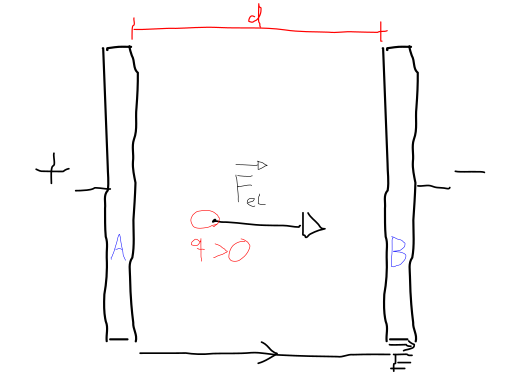
\includegraphics[width=\textwidth]{/home/daniel/documents/docs/LaTeX/notes/physic-figures/spdef-1.png}
\end{minipage}\hfill

\begin{minipage}[t]{0.45\textwidth}
\centering
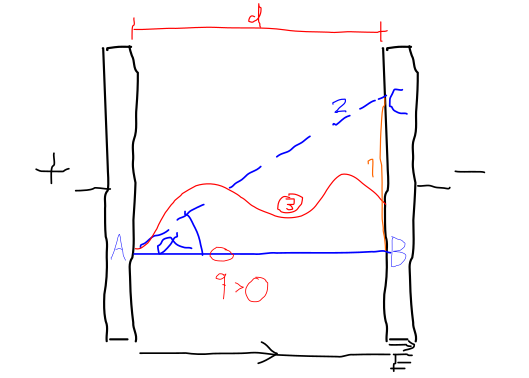
\includegraphics[width=\textwidth]{/home/daniel/documents/docs/LaTeX/notes/physic-figures/spdef-2.png}
\end{minipage}
\end{center}


\textbf{Allgemein gilt:} 
\begin{align*}
\Delta E&=F_{\parallel} \cdot s \\
\Delta E&=F_{\parallel} \cdot s = F \cdot s \cdot \cos(\alpha)
\end{align*}

\begin{enumerate}
  \item \[\Delta E_{BC}=F_{el} \cdot \overline{BC}\cdot \cos(90^{\circ})=0\]
  \item \[\Delta E_{AC}=F_{el} \cdot \overline{AC}\cdot \cos(\alpha)=\Delta E_{AB}\]
  \item l\"asst sich durch einen Polygonzug approximieren. F\"ur jedes Teilst\"uck gilt das Ergebnis (2). Ergebnis $\Delta E_{AB}$ ist unabh\"angig vom \"Ubertragungsweg.
\end{enumerate}


\begin{tcolorbox}[colback=red!10!white,colframe=red!80!black]
  F\"ur die elektrische Feldst\"arke im Homogenen Feld eines Plattenkondensators mit dem Plattenabstand $d$ gilt: $E=\frac{q}{d}; [E]=1\frac{N}{C}$.
\end{tcolorbox}


\begin{center}
%%\input{/home/daniel/documents/docs/LaTeX/notes/physic-figures/spannungdef3.tex}
\end{center}

\begin{tcolorbox}[colback=blue!10!white,colframe=blue!80!black]
  Ein Wattest\"uck hat die masse $m=0,01g$ und die Ladung $q=0,10nC$. Welche
  Geschwindigkeit w\"urde es erreichen, wenn es im Vakuum die Spannung
  $U=100kV$ durchliefe? Wie gros m\"usste die Spannung zwischen waagerecht
  liegenden Kondensatorplatten vom Abstand 20cm sein, damit das Wattest\"uck
  darin schwebt?
\end{tcolorbox}

\begin{figure}[htpb]
  \begin{center}
    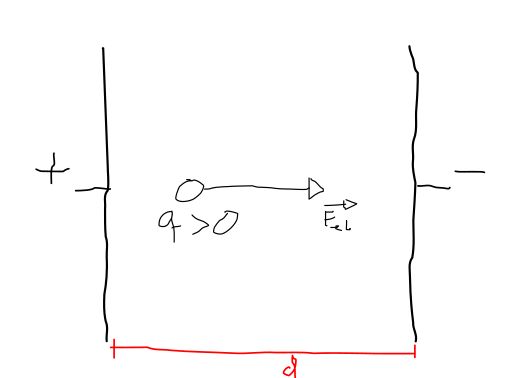
\includegraphics[width=0.5\textwidth]{/home/daniel/documents/docs/LaTeX/notes/physic-figures/spdef-3.png}
  \end{center}
  \caption{spdef-3}
\end{figure}


Ab dieser Aufgabe h\"ort es auf einen Sinn zu machen, auch die Rechnung
k\"onnte ein wenig verwirrt sein, da es so im Unterricht war.

$m=0,01g \quad =1\cdot 10^{-5}$\\
$q=0,10nC\quad =1,0\cdot 10^{-8}$\\
$U=100kV \quad =1,00\cdot 10^{5}$\\
$s=0,2m  \quad =20cm$

\begin{align*}
  &\dots\\
  VB&=\sqrt{2\cdot \frac{q}{m}\cdot U}\\
  VB&=\sqrt{2\cdot \frac{1,0\cdot 10^{-10}C}{1\cdot 10^{-5}kg}\cdot 1 \cdot 10^5V}\\
  &\approx 1 \frac{m}{s}\\
\end{align*}


\begin{figure}
  \begin{center}
    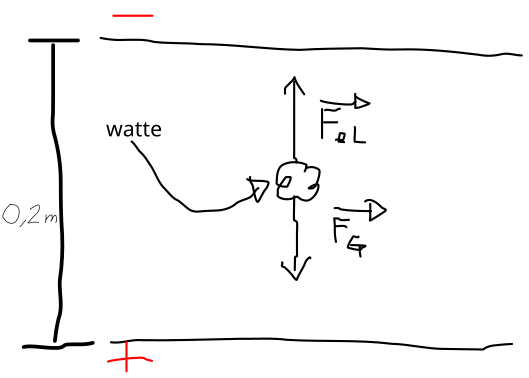
\includegraphics[width=0.5\textwidth]{/home/daniel/documents/docs/LaTeX/notes/physic-figures/spdef-4.png}
  \end{center}
  \caption{Watte}
  \label{fig:watte1}
\end{figure}



\begin{align*}
  F_{el}&=F_G\\
  \implies q\cdot E&=m\cdot g\\
  \implies q\cdot \frac{u}{d} &= m\cdot g\\
  \Leftrightarrow u&=\frac{m\cdot g \cdot d}{q}\\
  \implies u&=1,962\cdot 10^5V
\end{align*}



\section{Das eletrische Potential}

%\begin{figure}[htpb]
  %\begin{center}
    %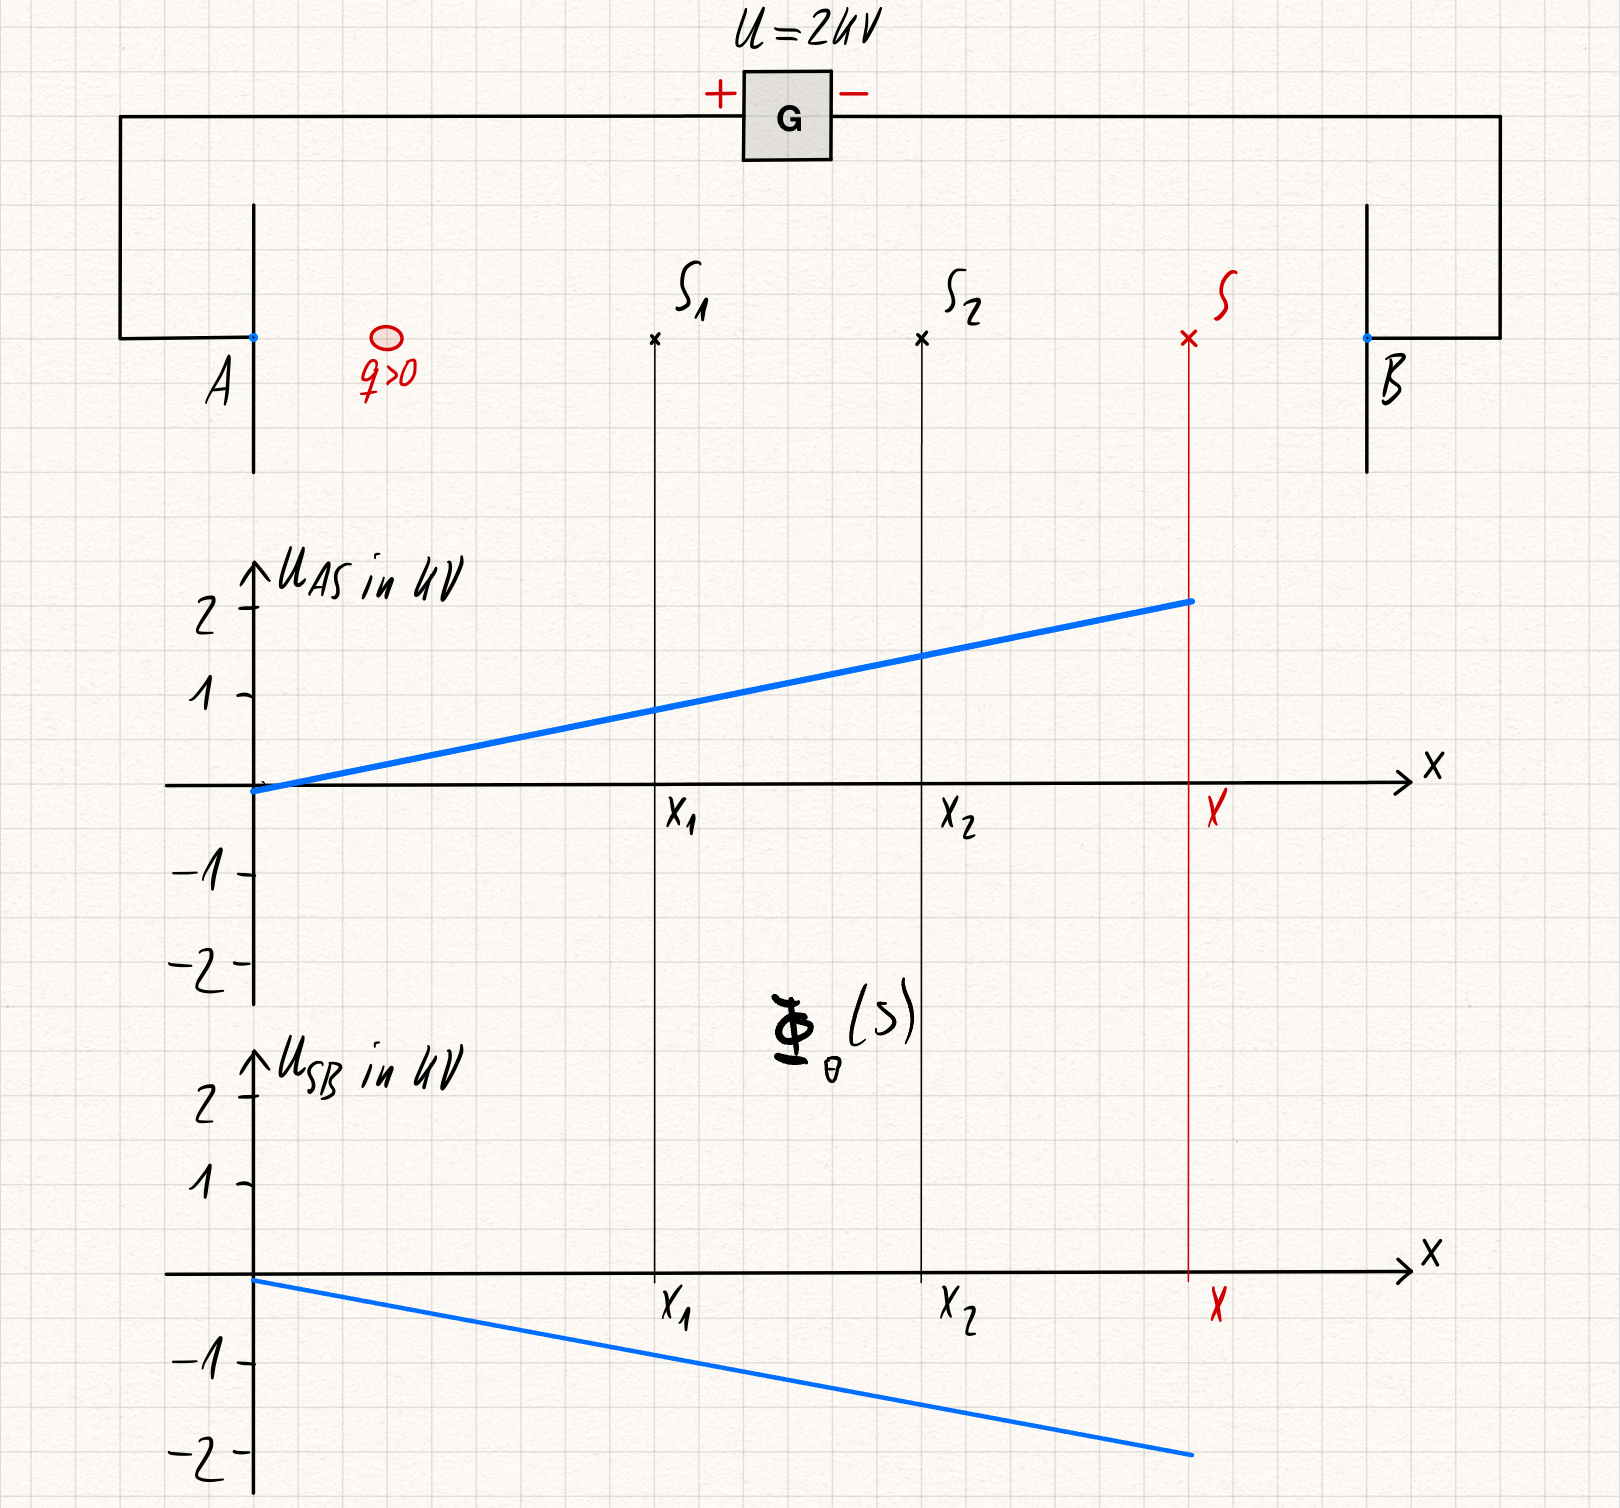
\includegraphics[width=0.5\textwidth]{/home/daniel/documents/docs/LaTeX/notes/physic-figures/skizze-potential.jpg}
  %\end{center}
%\end{figure}

Spannung $U_{AS}$ zwischen A und S:\\
\[U_{AS}=\frac{\Delta E_{AS}}{q}=\frac{F_{el}\cdot x}{q}=-E\cdot x +2\]


\begin{tcolorbox}[colback=yellow!10!white,colframe=yellow!80!black]

Die Spannung $U_{SB}$ von einem beliebigen Punkt $B$ heißt elektrisches
Potential $\Phi_B(S)$ des Punktes $S$ bezüglich $B$.
\[E \cdot (x_2 - x_1) = E\cdot \Delta x \]

Spannung $U_{S_1S_2}$ zwischen $S_1$ und $S_2$:

\[U_{S_1S_2}= \frac{\Delta E_{S_1S_2}}{q}=\frac{-\Delta E_{S_2A}-(-\Delta
E_{S_1A})}{q}=-\Phi_1(S_2)-(-\Phi_1(S_1))=\Delta\Phi_A(2) \quad (1)=(2):E \cdot
\Delta x=-\Delta\Phi_A\]

Eigenschaften des Potentials $\Phi$:
  \begin{enumerate}
    \item $\Phi$ nimmt in Feldrichtung ab.
    \item Die Spannung zwischen den Punkten $S_1$ und $S_2$ ist gleich ihrer Potentialdifferenz.
    \item \[E=\frac{\Delta\Phi_A}{\Delta x}, \text{ falls E konstant ist.}\]
    \[E=-\Phi'_A(x), \text{ falls E nicht konstant ist.}\]
  \end{enumerate}
\end{tcolorbox}



\begin{tcolorbox}[colback=gray!10!white,colframe=gray!80!black]
  \subsection{Hausaufgaben} \paragraph{A1:} 
  Zwischen zwei Kondensatorplatten mit $d=2$cm Abstand liegt die Spannung
  1,0kV. Wie gros ist die Feldstaerke $E$ wie gros die Kraft $F$ auf eine
  Probeladung $q=10$nC? Welche Energie wird von den Feldkraeften beim Transport
  von der einen zur anderen Platte aufgewandt? Pruefen Se die Spannungsangabe
  mit $U=\frac{W}{q}$ nach!



\paragraph{Loesung:}
Die Feldstärke $E$ kann mit der Formel $E=\frac{U}{d}$ berechnet werden:

\begin{equation*}
    E=\frac{U}{d}=\frac{1,0\mathrm{kV}}{2\mathrm{cm}}=50\mathrm{kV/m}
\end{equation*}

Die Kraft auf die Probeladung $F$ kann mit der Formel $F=q\cdot E$ berechnet werden:

\begin{equation*}
    F=q\cdot E=10\mathrm{nC}\cdot 50\mathrm{kV/m}=0,5\mathrm{\mu N}
\end{equation*}

Die Energie, die von den Feldkräften beim Transport von der einen zur anderen
Platte aufgewandt wird, kann mit der Formel $W=q\cdot U$ berechnet werden:

\begin{equation*}
    W=q\cdot U=10\mathrm{nC}\cdot 1,0\mathrm{kV}=10\mathrm{\mu J}
\end{equation*}

Um die Spannungsangabe mit $U=\frac{W}{q}$ zu prüfen, setzen wir die gegebenen Werte ein:

\begin{equation*}
    U=\frac{W}{q}=\frac{10\mathrm{\mu J}}{10\mathrm{nC}}=1,0\mathrm{kV}
\end{equation*}

Die Spannungsangabe ist also korrekt.
\end{tcolorbox}

\section{Wiederholung}

Coloumb ist nur f\"ur Punkladungen, nicht f\"ur Felder.
\[\left(F_{el}=\frac{1}{4\pi\epsilon_0}\cdot \frac{q_1\cdot q_2}{r^2}\right)\]

Irgendwas mit Probeladung: \[E=\frac{F_{el}}{q_{Probe}}\]

\textit{Des hier ist allgemein die Definiition f\"ur die elektrische Feldst\"arke.}
Im Kondensator f\"ur die Elektrische Feldstaerke braucht man nur
$E=\frac{U}{d}$, $\frac{Spannung}{Plattenabstand}$.


Die Ladungsdichte $\sigma$ ist Konstant, es ist die gedachte N\"ahe, der
Vektoren, Feldlinien und wie nah sie einander sind.

\textit{Definition von Sigma ($\sigma$):}
\[\sigma=\frac{q}{A} \quad =\frac{16e}{A} \quad = 16 \frac{e}{A} \quad = \frac{8e}{\frac{1}{2}A} \quad = 16 \frac{e}{A}\]

In einem Homogenen Feld soll an sich alles linear/proportional sein, wenn man
die Spannung verdoppelt, dann verdoppeltet sich die Dichte der Feld-Vektoren
$\sigma$ und auch die Feldspannung.

\begin{table}
  \caption{Irgendwas von der Tafel}
  \begin{center}
    \begin{tabular}[c]{l|l|l|l}
      \hline
      $\sigma$ & 16 & 30 & 56 \\
      \hline
      $E$ & $E_0$ & $2\cdot E_0$ & $4\cdot E_0$\\
      \hline
      $\frac{\sigma}{E}$ & $\frac{16}{E_0}$ & $\frac{15}{E_0}$ & $\frac{14}{E_0}$\\
    \end{tabular}
  \end{center}
\end{table}

\subsection{Flaechenladungsdichte und elektrische Felstaerke im homogenen Feld}

\begin{tcolorbox}[colback=red!10!white,colframe=red!75!black]
Auf einer Ebenem Flaeche mit inhalt $A$ verteilt sich eine Ladungsmenge $Q$ in
der Regel gleichmaesig. Die Flaechendichte $\sigma$ gibt an, wie dicht die
Ladungen auf dieser Fl\"ache sitzen. Sie berechnet sich bei einer
gleichm\"asigen Ladungsvertailung \"uber \[\sigma = \frac{Q}{A}; [\sigma]=1
\frac{C}{m^2}.\]
\end{tcolorbox}

Vergr\"osern wir die eletkrische Feldst\"arke im Plattenkondensator, indem wir
entweder die Spannung $U$ erh\"ohen oder den Plattenabstand $d$ verringern, so
stellen wir fest, dass \[\sigma ~ E\] gilt. \[\implies \frac{\sigma}{E}=konstant=\epsilon_0\]

\begin{tcolorbox}[colback=red!10!white,colframe=red!75!black]
Die Feldst\"arke $E$ eines homogenen Feldes ist proportional zur
Fl\"achenladungsdichte $\sigma$ der sie erzeugenden Ladung. In Luft gilt
\[\sigma = \epsilon_0 \cdot E\] \textit{Hier ist $\sigma$ Ursache des Feldes und $E$ die Wirkung.}\\
mit der elektrischen Feldkonstanten \[\epsilon_0 = 8,85 \cdot 10^{12} \frac{C^2}{Nm^2}\]
\end{tcolorbox}


\section{Planarbeit: Plattenkondensator}
\subsection{Vorbereitung}
\textbf{Von welchen Gr\"osen k\"onnte die Ladungsmenge, die in einem
Plattekondensator gespeichert ist ab?}

\textit{Ziele: }
\begin{itemize}
  \item Die Definition der Kapazität eines Kondensators kennen, verstehen und anwenden können.
  \item Die Formel zur Berechnung der Kapazität eines Plattenkondensators kennen, verstehen und anwenden können.
  \item Den Einfluss von Dielektrika in Kondensatoren kennen und verstehen.
\end{itemize}

Die Kapazität eines Kondensators ist ein Maß für die Fähigkeit des
Kondensators, elektrische Ladung zu speichern. Es wird gemessen in Farad (F).
Ein Kondensator mit einer Kapazität von 1 Farad kann eine elektrische Ladung
von 1 Coulomb speichern, wenn eine Spannung von 1 Volt angelegt wird.


Die Ladung $Q$ auf einem Kondensator ist der Spannung U zwischen den Platten
proportional. Unter der Kapazitat $C$ eines Kondensator versteht man den
Quotienten.
\[C=\frac{Q}{U}; \quad \text{Einheit:} [C]=1 \frac{C}{V} = 1F (Farad).\]

Fuer einen Plattenkondensator mit Flaeche $A$ und Abstand $d$ gilt: 
\[C=\epsilon_0 \cdot \frac{A}{d}.\]



Ein Kondensator besteht aus zwei leitenden Platten, die durch ein Dielektrikum
getrennt sind. Wenn eine Spannung an den Platten anliegt, werden elektrische
Ladungen auf den Platten gespeichert, wodurch ein elektrisches Feld im
Dielektrikum erzeugt wird. Das Dielektrikum beeinflusst die Kapazität des
Kondensators, indem es die elektrische Feldstärke zwischen den Platten
reduziert und somit die elektrische Ladung, die auf den Platten gespeichert
werden kann, erhöht.

Durch die Verwendung von Dielektrika mit höherer Dielektrizitätskonstante kann
die Kapazität des Kondensators erhöht werden. Dielektrika können auch dazu
beitragen, die Spannungsfestigkeit des Kondensators zu erhöhen, indem sie das
elektrische Feld zwischen den Platten besser isolieren und somit ein
Durchschlagen verhindern. Die Eigenschaften des Dielektrikums beeinflussen
somit maßgeblich die Leistung und Funktionalität des Kondensators.


\textbf{Permittivit\"at}
Die relative Permittivit\"at $\epsilon_0$ gibt die Erhoehung der Kapazitaet
durch ein Dielektrikum an. Im Vakuum ist $\epsilon_r$ gibt die Ehoehung der
Kaoazitat durch ein Dielektrikum an. Im Vakuum ist $\epsilon_r = 1$. Die
Kapazitaet eines Plattenkondensators mit der Fl\"ache $A$ und dem
Plattenabstand $d$ ist
\[C=\epsilon_r \cdot \epsilon_0 \cdot \frac{A}{d}.\]

\subsubsection{Aufgabe}
\textbf{2}, \textit{Berechnen sie die kapazitat C eines Kondensators mit Ladungsmenge
$Q=10nC$ und einer angelegten Spannung con $U=5V$}
\[ C=\frac{Q}{U} \quad \implies \quad \frac{10 \cdot 10^{-9}}{5}= 2\cdot 10^{-10} \]

Berechnen sie die Ladungsmenge eines Kondensators mit der Kapazitaet 1000 $\mu
F$ und einer angelegten spannung von 3,3V Also 0,001 Farad (C).
\[
  C \dot U = Q \quad \implies \quad 0,001\cdot 3,3= 0.003 C
\]

\textbf{3}
Hier nochmal die formel: $C=\epsilon_r \cdot \epsilon_0 \cdot \frac{A}{d}$,
daraus muss man entweder $\epsilon_r$ verhundertfachen, oder $A$ da sie
Faktoren sind, man kann aber auch $d$, weil es ein Quotient ist durch hundert
rechnen.

\textbf{4}
Stellen Sie eine Formel auf, die den Zusammenhang zwischen der elektrischen
Feldstaerke eines Plattenkondensators und seiner Kapazitaet wiedergibt.

\textbf{5}
Bestimmen sie die Kapazitaet eine Kondensators unter Zuhlifenahme eines
Diagramms mit folgenden Messwerten:

\begin{table}[htpb]
  \begin{center}
    \begin{tabular}{|l|l|l|l|l|}
      \hline
      \textbf{$U$ in $V$} & 50 & 100 & 150 & 200 \\
      \hline
      \textbf{$Q$ in $nC$}& 11 &  21 &  29 &  41 \\
      \hline
    \end{tabular}
  \end{center}
\end{table}


\section{Winkel und Kreisbewegungen?}
\subsection{Vertiefung}
skalare sind
\begin{enumerate}
  \item die umlaufdauer $T$ und 
  \item Die drehfrequenz
\end{enumerate}

Vektorielle groesen sind
\begin{enumerate}
  \item Der Radiusvektor $\vec{r}$ von der Drehachse zum Koerper.\\
    \textit{Man denke sich hier ein Kreis, welcher punkte au\ss~en hat, ivon
    dem Mittelpunkt aus zeigt der Vektor auf die Punkte, am Kreis verteilt. Der
    Radiusvektor zeeigt zu drei verschiedenen zieten auf die verschiedenen
    Punkte, der Kreis bewegt sich im Uhrzeigersinn und ist nicht Konstant, Betrag
    (Laenge des Vektors) ist Konstant aber die Richtung ist entscheident.}
  \item die Bahngeschwindigkeit $\vec{v}$ des Koerpers $K$ ist am voherigen
    Kreis, Tangential des Kreises entlang, in Richtung der Bewegung.
    Die Bahngeschwindigkeit ist ueberall am Kreis gleich lang, da der Kreis
    nicht anders schnell sein kann am gleichen Kreis, die Tangenten haben auch
    immer rechte Winkel zum Kreis-inneren.
    (Richtung aendert sich staendig, betrag bleibt meist gleich)

    wegen $|\vec{v}|=v=2\pi\cdot r\cdot f= \text{konstant}$  handelt es sich um
    eine gleichfoermige kreisbewegung.
  \item \textit{Hier aus dem iPad einfuegen}, \textbf{Die Winkelgeschwindigkeit $\vec{\omega}$} 
\end{enumerate}
\paragraph{Dynamik der Kreisbewegung}
Fuert ein Koerper eine \textbf{gleichfoermige Kreisbewegung} ($|\vec{v}|$=
konstant) aus, so wirkt auf ihn in jedem Bahnpunkt eine zum Kreismittelpunkt
gerichtete \textbf{Zentripeltalkraft $\vec{F_Z}$}, diese zwingt den Koerper auf
die Kreisbahn. 

\clearpage

\subsection{Deduktion einer Formel fuer den Betrag von $\vec{F_Z}$}
Wegen $F_Z = m \cdot a_Z$ leiten wir zunachst eine gleichung fuer $a_Z$ her.

\begin{figure}[htpb]
  \begin{center}
    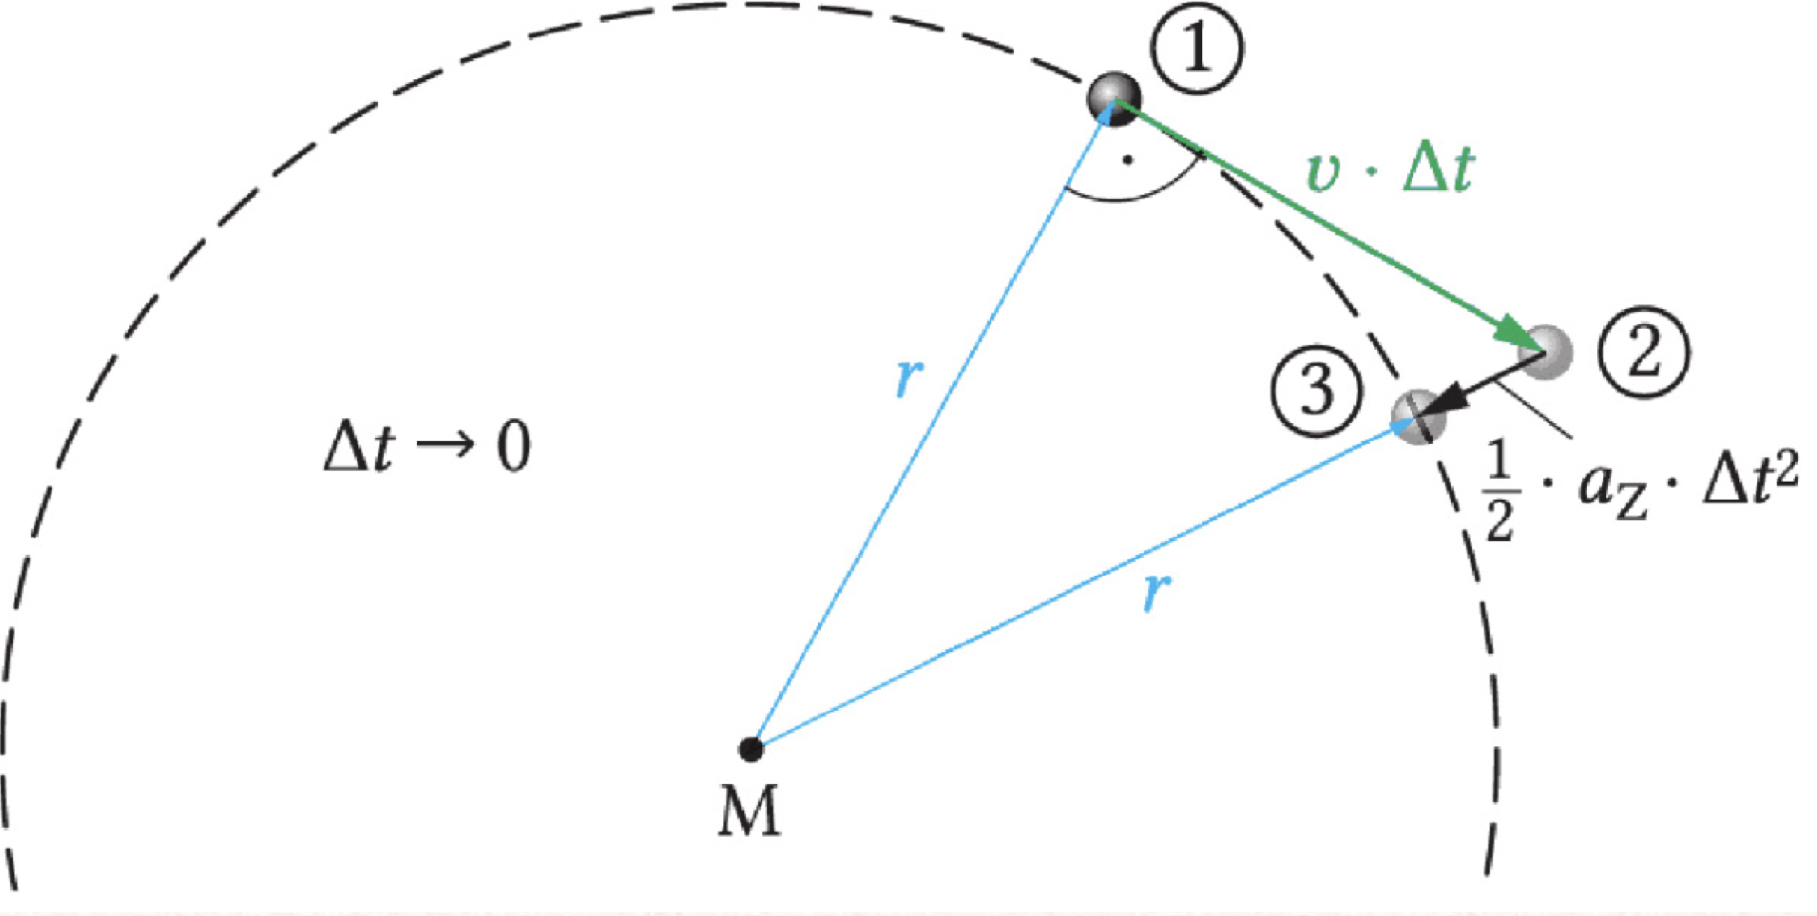
\includegraphics[width=0.5\textwidth]{./physic-figures/kreisbewegung.jpg}
  \end{center}
  \caption{Abbildung aus dem Buch}
\end{figure}


Ziel ist es eine gleichung zu finden, die $a_Z$ enthealt. 

Von $1$ bis $2$ gleichmaesig Bewegung tangential zur Kreisbahn.

Von $2$ bis $3$ gleichmaesig beschleunigte Bewegung in Richtung Kreismittelpunkt.

Da das ($\Delta M$ \textcircled{1}\textcircled{2}) rechtwinklig ist, folgt aus dem Satz des Pythagoras.

\begin{multicols}{2}
\begin{align*}
  r^2 + (v\cdot \Delta t)^2 &= (r+\frac{1}{2}a_2\Delta t^2)^2\\
  \Leftrightarrow r^2+v^2 \cdot \Delta t^2 &=r^2+2\cdot r \cdot \frac{1}{2} \cdot a_2 \Delta t^2+\frac{1}{a}a_2 \cdot \Delta t^4\\
  \Leftrightarrow v\cdot \Delta t^2&= r\cdot a_2 \cdot \Delta t^2 + \frac{1}{4} a_Z^2 \cdot \Delta t^4\\
  \Leftrightarrow v^2 &=r\cdot a_Z + \frac{1}{4}a_Z^2 \cdot \Delta t^2\\
  \text{mit $\Delta t \to 0$ folgt}&\\
  v^2&=r\cdot a_Z\\
  \Leftrightarrow a_Z &=\frac{v^2}{r}\\
  \implies F_Z &=m\cdot a_Z = m\cdot \frac{v^2}{r}\\
\end{align*}

\begin{align*}
  a(t)&=a=\text{konstant}\\
  a(t)&=v'(t)\\
  v(t)&=a\cdot t+v_0\\
  v(t)&=s'(t)\\
  s'(t)&=\frac{1}{2}a\cdot t^2+v_0\cdot t + s_0
\end{align*}

\begin{align*}
  \vec{F_Z}&=m\cdot \vec{a_Z}\\
  F_Z&=m\cdot a_Z\\
  f''(x)&=2 | a\\
  f'(x)&=2x | a\cdot x \\
  f(x)&=x^2\\
\end{align*}
\end{multicols}

\clearpage

\paragraph{Strategie:}
\begin{itemize}
  \item Damit ein Koerper eine Kreisbewegung ausfuert, ist eine zum
    Kreismittelpunkt gerichtete Zentripetalkraft, $\vec{F_Z}$ erforderlich. 
  \item Diese ist die \textbf{Resultierende} aller Koerper angreifenden Kraefte.
  \item Man ueberlegt sich also immer zuerst welche aeuseren Kraefte am Koerper angreifen.
\end{itemize}


\begin{figure}[htpb]
  \begin{center}
    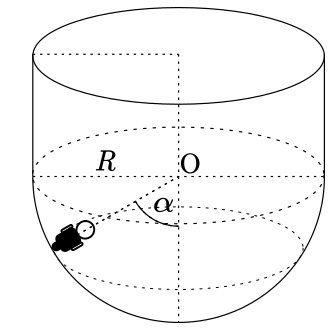
\includegraphics[width=0.3\textwidth]{./physic-figures/steil.png}
  \end{center}
  \caption{Steile Wand}
\end{figure}
\paragraph{Beispiel:}
Pitt’s Todeswand hat einen Durchmesser von 12,0 m. Die
Reibungszahl zwischen dem Holzboden und den Rädern des Motorrads
unterschreitet den Wert 0, 30 nicht.
Berechnen Sie, mit welcher Geschwindigkeit die Steilwandfahrerin min-
destens fahren muss, damit sie in der senkrechten Wand ihre Runden
drehen kann.

\paragraph{Aufgabe:}
Die in der Abbildung skizzierte Steil-
wandarena hat die Form einer Halbkugel mit
dem Mittelpunkt O und dem Radius R “ 10 m
mit aufgesetztem Zylinder. Der Steilwandfahrer
und das Motorrad haben zusammen die Masse
$m = 200 kg$.

Der Steilwandfahrer bewegt sich im unteren Teil
der Arena mit seinem Motorrad auf einer horizon-
talen Kreisbahn. Motorrad und Fahrer befinden
sich dabei in jedem Augenblick senkrecht zur Wand.
Der Schwerpunkt von Motorrad und Fahrer hat
von O näherungsweise die Entfernung 10 m. Die
Winkelweite α beträgt 60˝.

\textbf{a)} Fertigen Sie eine maßstäbliche Skizze mit den
im Schwerpunkt angreifenden Kräften an.
Erläutern Sie anhand Ihrer Skizze, wie in die-
sem Fall die erforderliche Zentripetalkraft zu-
stande kommt.

\textbf{b)} Berechnen Sie den Betrag der Zentripetalkraft,
die für eine stabile Kreisbewegung des Steil-
wandfahrers notwendig ist.

\textbf{c)} Berechnen Sie schließlich die Bahngeschwin-
digkeit des Steilwandfahrers.








\clearpage
\section{box tests}
\tbox{test}
\regel{test}
\nt{test}
\ex{test}
\q{test}


\end{document}
